\documentclass[a4paper]{article}

\def\npart {IB}
\def\nterm {Lent}
\def\nyear {2016}
\def\nlecturer {P. F. Linden}
\def\ncourse {Fluid Dynamics}

% Imports
\ifx \nextra \undefined
  \usepackage[pdftex,
    hidelinks,
    pdfauthor={Dexter Chua},
    pdfsubject={Cambridge Maths Notes: Part \npart\ - \ncourse},
    pdftitle={Part \npart\ - \ncourse},
  pdfkeywords={Cambridge Mathematics Maths Math \npart\ \nterm\ \nyear\ \ncourse}]{hyperref}
  \title{Part \npart\ - \ncourse}
\else
  \usepackage[pdftex,
    hidelinks,
    pdfauthor={Dexter Chua},
    pdfsubject={Cambridge Maths Notes: Part \npart\ - \ncourse\ (\nextra)},
    pdftitle={Part \npart\ - \ncourse\ (\nextra)},
  pdfkeywords={Cambridge Mathematics Maths Math \npart\ \nterm\ \nyear\ \ncourse\ \nextra}]{hyperref}

  \title{Part \npart\ - \ncourse \\ {\Large \nextra}}
\fi

\author{Lectured by \nlecturer \\\small Notes taken by Dexter Chua}
\date{\nterm\ \nyear}

\usepackage{alltt}
\usepackage{amsfonts}
\usepackage{amsmath}
\usepackage{amssymb}
\usepackage{amsthm}
\usepackage{booktabs}
\usepackage{caption}
\usepackage{enumitem}
\usepackage{fancyhdr}
\usepackage{graphicx}
\usepackage{mathtools}
\usepackage{microtype}
\usepackage{multirow}
\usepackage{pdflscape}
\usepackage{pgfplots}
\usepackage{siunitx}
\usepackage{tabularx}
\usepackage{tikz}
\usepackage{tkz-euclide}
\usepackage[normalem]{ulem}
\usepackage[all]{xy}

\pgfplotsset{compat=1.12}

\pagestyle{fancyplain}
\lhead{\emph{\nouppercase{\leftmark}}}
\ifx \nextra \undefined
  \rhead{
    \ifnum\thepage=1
    \else
      \npart\ \ncourse
    \fi}
\else
  \rhead{
    \ifnum\thepage=1
    \else
      \npart\ \ncourse\ (\nextra)
    \fi}
\fi
\usetikzlibrary{arrows}
\usetikzlibrary{decorations.markings}
\usetikzlibrary{decorations.pathmorphing}
\usetikzlibrary{positioning}
\usetikzlibrary{fadings}
\usetikzlibrary{intersections}
\usetikzlibrary{cd}

\newcommand*{\Cdot}{\raisebox{-0.25ex}{\scalebox{1.5}{$\cdot$}}}
\newcommand {\pd}[2][ ]{
  \ifx #1 { }
    \frac{\partial}{\partial #2}
  \else
    \frac{\partial^{#1}}{\partial #2^{#1}}
  \fi
}

% Theorems
\theoremstyle{definition}
\newtheorem*{aim}{Aim}
\newtheorem*{axiom}{Axiom}
\newtheorem*{claim}{Claim}
\newtheorem*{cor}{Corollary}
\newtheorem*{defi}{Definition}
\newtheorem*{eg}{Example}
\newtheorem*{fact}{Fact}
\newtheorem*{law}{Law}
\newtheorem*{lemma}{Lemma}
\newtheorem*{notation}{Notation}
\newtheorem*{prop}{Proposition}
\newtheorem*{thm}{Theorem}

\renewcommand{\labelitemi}{--}
\renewcommand{\labelitemii}{$\circ$}
\renewcommand{\labelenumi}{(\roman{*})}

\let\stdsection\section
\renewcommand\section{\newpage\stdsection}

% Strike through
\def\st{\bgroup \ULdepth=-.55ex \ULset}

% Maths symbols
\newcommand{\bra}{\langle}
\newcommand{\ket}{\rangle}

\newcommand{\N}{\mathbb{N}}
\newcommand{\Z}{\mathbb{Z}}
\newcommand{\Q}{\mathbb{Q}}
\renewcommand{\H}{\mathbb{H}}
\newcommand{\R}{\mathbb{R}}
\newcommand{\C}{\mathbb{C}}
\newcommand{\Prob}{\mathbb{P}}
\renewcommand{\P}{\mathbb{P}}
\newcommand{\E}{\mathbb{E}}
\newcommand{\F}{\mathbb{F}}
\newcommand{\cU}{\mathcal{U}}
\newcommand{\RP}{\mathbb{RP}}
\newcommand{\CP}{\mathbb{CP}}

\newcommand{\ph}{\,\cdot\,}

\DeclareMathOperator{\sech}{sech}
\DeclareMathOperator{\cosech}{cosech}
\DeclareMathOperator{\cosec}{cosec}

\DeclareMathOperator{\covol}{covol}
\DeclareMathOperator{\vol}{vol}

\let\Im\relax
\let\Re\relax
\DeclareMathOperator{\Im}{Im}
\DeclareMathOperator{\Re}{Re}
\DeclareMathOperator{\im}{im}
\DeclareMathOperator{\image}{image}
\DeclareMathOperator{\Ann}{Ann}

\DeclareMathOperator*{\res}{res}
\DeclareMathOperator{\Res}{Res}
\DeclareMathOperator{\Ind}{Ind}

\DeclareMathOperator{\tr}{tr}
\DeclareMathOperator{\diag}{diag}
\DeclareMathOperator{\rank}{rank}
\DeclareMathOperator{\card}{card}
\DeclareMathOperator{\spn}{span}
\DeclareMathOperator{\adj}{adj}

\DeclareMathOperator{\erf}{erf}
\DeclareMathOperator{\erfc}{erfc}

\DeclareMathOperator{\ord}{ord}
\DeclareMathOperator{\Sym}{Sym}

\DeclareMathOperator{\sgn}{sgn}
\DeclareMathOperator{\orb}{orb}
\DeclareMathOperator{\stab}{stab}
\DeclareMathOperator{\ccl}{ccl}

\DeclareMathOperator{\lcm}{lcm}
\DeclareMathOperator{\hcf}{hcf}

\DeclareMathOperator{\Int}{Int}
\DeclareMathOperator{\id}{id}

\DeclareMathOperator{\betaD}{beta}
\DeclareMathOperator{\gammaD}{gamma}
\DeclareMathOperator{\Poisson}{Poisson}
\DeclareMathOperator{\binomial}{binomial}
\DeclareMathOperator{\multinomial}{multinomial}
\DeclareMathOperator{\Bernoulli}{Bernoulli}
\DeclareMathOperator{\like}{like}

\DeclareMathOperator{\var}{var}
\DeclareMathOperator{\cov}{cov}
\DeclareMathOperator{\bias}{bias}
\DeclareMathOperator{\mse}{mse}
\DeclareMathOperator{\corr}{corr}

\DeclareMathOperator{\otp}{otp}
\DeclareMathOperator{\dom}{dom}

\DeclareMathOperator{\Root}{Root}
\DeclareMathOperator{\supp}{supp}
\DeclareMathOperator{\rel}{rel}
\DeclareMathOperator{\Hom}{Hom}
\DeclareMathOperator{\Aut}{Aut}
\DeclareMathOperator{\Gal}{Gal}
\DeclareMathOperator{\Mat}{Mat}
\DeclareMathOperator{\End}{End}
\DeclareMathOperator{\Char}{char}
\DeclareMathOperator{\ev}{ev}
\DeclareMathOperator{\St}{St}
\DeclareMathOperator{\Lk}{Lk}
\DeclareMathOperator{\disc}{disc}
\DeclareMathOperator{\Isom}{Isom}
\DeclareMathOperator{\length}{length}
\DeclareMathOperator{\energy}{energy}
\DeclareMathOperator{\area}{area}
\DeclareMathOperator{\Syl}{Syl}
\DeclareMathOperator{\cl}{cl}
\DeclareMathOperator{\fix}{fix}

\newcommand{\GL}{\mathrm{GL}}
\newcommand{\SL}{\mathrm{SL}}
\newcommand{\PGL}{\mathrm{PGL}}
\newcommand{\PSL}{\mathrm{PSL}}
\newcommand{\PSU}{\mathrm{PSU}}
\newcommand{\Or}{\mathrm{O}}
\newcommand{\SO}{\mathrm{SO}}
\newcommand{\U}{\mathrm{U}}
\newcommand{\SU}{\mathrm{SU}}

\renewcommand{\d}{\mathrm{d}}
\newcommand{\D}{\mathrm{D}}

\tikzset{->/.style = {decoration={markings,
                                  mark=at position 1 with {\arrow[scale=2]{latex'}}},
                      postaction={decorate}}}
\tikzset{<-/.style = {decoration={markings,
                                  mark=at position 0 with {\arrowreversed[scale=2]{latex'}}},
                      postaction={decorate}}}
\tikzset{<->/.style = {decoration={markings,
                                   mark=at position 0 with {\arrowreversed[scale=2]{latex'}},
                                   mark=at position 1 with {\arrow[scale=2]{latex'}}},
                       postaction={decorate}}}
\tikzset{->-/.style = {decoration={markings,
                                   mark=at position #1 with {\arrow[scale=2]{latex'}}},
                       postaction={decorate}}}
\tikzset{-<-/.style = {decoration={markings,
                                   mark=at position #1 with {\arrowreversed[scale=2]{latex'}}},
                       postaction={decorate}}}

\tikzset{circ/.style = {fill, circle, inner sep = 0, minimum size = 3}}
\tikzset{mstate/.style={circle, draw, blue, text=black, minimum width=0.7cm}}

\definecolor{mblue}{rgb}{0.2, 0.3, 0.8}
\definecolor{morange}{rgb}{1, 0.5, 0}
\definecolor{mgreen}{rgb}{0.1, 0.4, 0.2}
\definecolor{mred}{rgb}{0.5, 0, 0}

\def\drawcirculararc(#1,#2)(#3,#4)(#5,#6){%
    \pgfmathsetmacro\cA{(#1*#1+#2*#2-#3*#3-#4*#4)/2}%
    \pgfmathsetmacro\cB{(#1*#1+#2*#2-#5*#5-#6*#6)/2}%
    \pgfmathsetmacro\cy{(\cB*(#1-#3)-\cA*(#1-#5))/%
                        ((#2-#6)*(#1-#3)-(#2-#4)*(#1-#5))}%
    \pgfmathsetmacro\cx{(\cA-\cy*(#2-#4))/(#1-#3)}%
    \pgfmathsetmacro\cr{sqrt((#1-\cx)*(#1-\cx)+(#2-\cy)*(#2-\cy))}%
    \pgfmathsetmacro\cA{atan2(#2-\cy,#1-\cx)}%
    \pgfmathsetmacro\cB{atan2(#6-\cy,#5-\cx)}%
    \pgfmathparse{\cB<\cA}%
    \ifnum\pgfmathresult=1
        \pgfmathsetmacro\cB{\cB+360}%
    \fi
    \draw (#1,#2) arc (\cA:\cB:\cr);%
}
\newcommand\getCoord[3]{\newdimen{#1}\newdimen{#2}\pgfextractx{#1}{\pgfpointanchor{#3}{center}}\pgfextracty{#2}{\pgfpointanchor{#3}{center}}}

\def\Xint#1{\mathchoice
   {\XXint\displaystyle\textstyle{#1}}%
   {\XXint\textstyle\scriptstyle{#1}}%
   {\XXint\scriptstyle\scriptscriptstyle{#1}}%
   {\XXint\scriptscriptstyle\scriptscriptstyle{#1}}%
   \!\int}
\def\XXint#1#2#3{{\setbox0=\hbox{$#1{#2#3}{\int}$}
     \vcenter{\hbox{$#2#3$}}\kern-.5\wd0}}
\def\ddashint{\Xint=}
\def\dashint{\Xint-}


\begin{document}
\maketitle
{\small
\noindent\textbf{Parallel viscous flow}\\
Plane Couette flow, dynamic viscosity. Momentum equation and boundary conditions. Steady flows including Poiseuille flow in a channel. Unsteady flows, kinematic viscosity, brief description of viscous boundary layers (skin depth).\hspace*{\fill} [3]

\vspace{10pt}
\noindent\textbf{Kinematics}\\
Material time derivative. Conservation of mass and the kinematic boundary condition. Incompressibility; streamfunction for two-dimensional flow. Streamlines and path lines.\hspace*{\fill} [2]

\vspace{10pt}
\noindent\textbf{Dynamics}\\
Statement of Navier-Stokes momentum equation. Reynolds number. Stagnation-point flow; discussion of viscous boundary layer and pressure field. Conservation of momentum; Euler momentum equation. Bernoulli's equation.

\vspace{5pt}
\noindent Vorticity, vorticity equation, vortex line stretching, irrotational flow remains irrotational. \hspace*{\fill} [4]

\vspace{10pt}
\noindent\textbf{Potential flows}\\
Velocity potential; Laplace's equation, examples of solutions in spherical and cylindrical geometry by separation of variables. Translating sphere. Lift on a cylinder with circulation.

\vspace{5pt}
\noindent Expression for pressure in time-dependent potential flows with potential forces. Oscillations in a manometer and of a bubble.\hspace*{\fill} [3]

\vspace{10pt}
\noindent\textbf{Geophysical flows}\\
Linear water waves: dispersion relation, deep and shallow water, standing waves in a container, Rayleigh-Taylor instability.

\vspace{5pt}
\noindent Euler equations in a rotating frame. Steady geostrophic flow, pressure as streamfunction. Motion in a shallow layer, hydrostatic assumption, modified continuity equation. Conservation of potential vorticity, Rossby radius of deformation.\hspace*{\fill} [4]}

\tableofcontents
\setcounter{section}{-1}
\section{Introduction}
In real life, we encounter a lot of fluids. For example, there is air and water. These are known as \emph{Newtonian fluids}, whose dynamics follow relatively simple equations. This is fundamentally because they have simple composition --- they are made up of simple molecules. An example of \emph{non-Newtonian} fluid is shampoo, which, despite looking innocent, has long chain molecules with complex properties.

In fluid dynamics, one of the most important things is to distinguish what is a fluid and what is not. For example, air and water are fluids, while the wall is solid. A main distinction is that we can lean on the wall, but not on air and water. In particular, if we apply a force on the wall, it will deform a bit, but then stop. A finite force on a solid will lead to a finite deformation. On the other hand, if we attempt to apply a force onto air or water, it will just move along the direction of force indefinitely. A finite force can lead to infinite deformation.

This is the main difference between solid mechanics and fluid mechanics. In solid mechanics, we look at properties like elasticity. This measures how much deformation we get when we apply a force. In fluid mechanics, we don't measure distances, since they can potentially be infinite. Instead, we would often be interested in the velocity of fluids.

There are many applications of fluid dynamics. On a small scale, the dynamics of fluids in cells is important for biology. On a larger scale, the fluid flow of the mantle affects the movement of tectonic plates, while the dynamics of the atmosphere can be used to explain climate and weather. On an even larger scale, we can use fluid dynamics to analyse the flow of galactic systems in the universe.

\section{Parallel viscous flow}
\setcounter{subsection}{-1}
\subsection{Preliminaries}
This section is called preliminaries, not definitions, because the ``definitions'' we give will be a bit fuzzy. We will (hopefully) get better definitions later on.

We start with an absolutely clear an unambiguous definition of the subject we are going to study.
\begin{defi}[Fluid]
  A \emph{fluid} is a material that flows.
\end{defi}

\begin{eg}
  Air, water and oil are fluids. These are known as \emph{simple} or \emph{Newtonian} fluids, because they are simple.

  Paint, toothpaste and shampoo are \emph{complex} or \emph{non-Newtonian} fluids, because they are complicated.

  Sand, rice and foams are \emph{granular flows}. These have some fluid-like properties, but are fundamentally made of small granular solids.
\end{eg}

In this course, we will restrict our attention to Newtonian fluids. Practically speaking, these are fluids for which our equations work. The assumption we will make when deriving our equations will be the following:

\begin{defi}[Newtonian fluids and viscosity]
  A \emph{Newtonian fluid} is a fluid with a linear relationship between stress and rate of strain. The constant of proportionality is \emph{viscosity}.
\end{defi}
This, and other concepts we define here, will become more clear when we start to write down our equations.

\begin{defi}[Stress]
  \emph{Stress} is force per unit area.
\end{defi}
For example, pressure is a stress.

\begin{defi}[Strain]
  \emph{Strain} is the extension per unit length. The \emph{rate of strain} is $\frac{\d}{\d t}(\mathrm{strain})$ is concerned with gradients of velocity.
\end{defi}
As mentioned in the introduction, for fluid dynamics, we tend to study velocities instead of displacements. So we will mostly work with rate of strain instead of strain itself.

These quantities are in fact tensor fields, but we will not treat them as such in this course. We will just consider ``simplified'' cases. For the full-blown treatment with tensor fields, refer to the IID Fluid Dynamics.

In this course, we are going make a lot of simplifying assumptions, since the world is too complicated. For example, most of the time, we will make the \emph{inviscid approximation}, where we set the viscosity to $0$. We will also often consider motions in one direction only.

\subsection{Stress}
We first look at stresses. These are the forces that exist inside the fluid. If we have a boundary, we can classify the stress according to the direction of the force --- whether it is normal to or parallel to the boundary. Note that the boundary can either be an actual physical boundary, or an imaginary surface we cook up in order to compute things.

Suppose we have a fluid with pressure $p$ acting on a surface with unit normal $\mathbf{n}$, pointing \emph{into} the fluid. This causes
\begin{center}
  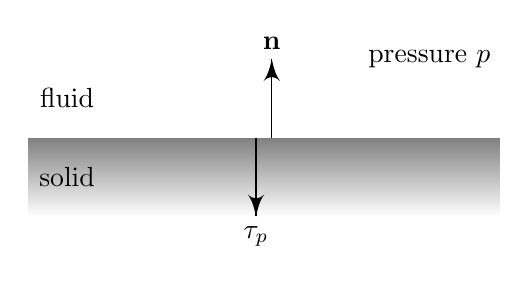
\begin{tikzpicture}
    \fill [gray, path fading=south] (0, 0) rectangle (6, -1);
    \draw [->] (3.1, 0) -- +(0, 1) node [above] {$\mathbf{n}$};
    \draw [->] (2.9, 0) -- +(0, -1) node [below] {$\tau_p$};
    \node at (0.5, -0.5) {solid};
    \node at (0.5, 0.5) {fluid};
    \node at (6, 1) [left] {pressure $p$};
  \end{tikzpicture}
\end{center}

\begin{defi}[Normal stress]
  The \emph{normal stress} is
  \[
    \tau_p = -p\mathbf{n}.
  \]
\end{defi}
The normal stress is present everywhere, as long as we have a fluid (with pressure). However, pressure by itself does not do anything, since pressure acts in all directions, and the net effect cancels out. However, if we have a pressure \emph{gradient}, then gives an actual force and drives fluid flow. For example, suppose we have a pipe, with the pump on the left:
\begin{center}
  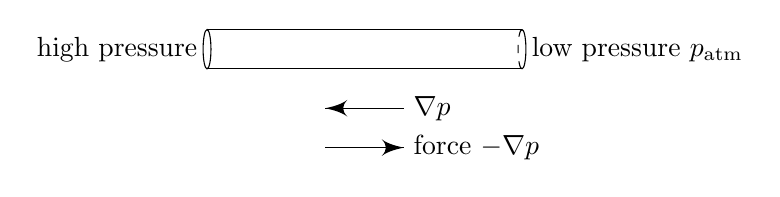
\begin{tikzpicture}
    \draw (0, 0) -- +(4, 0);
    \node at (0, 0.25) [left] {high pressure};
    \node at (4, 0.25) [right] {low pressure $p_{\mathrm{atm}}$};
    \draw (0, 0.5) -- +(4, 0);
    \draw [->] (2.5, -0.5) node [right] {$\nabla p$} -- +(-1, 0);
    \draw [->] (1.5, -1) -- +(1, 0) node [right] {force $-\nabla p$};
    \draw (0, 0.25) ellipse (0.05 and 0.25);
    \draw [dashed] (4, 0) arc (270:90:0.05 and 0.25);
    \draw (4, 0) arc (270:450:0.05 and 0.25);
  \end{tikzpicture}
\end{center}
Then this gives a \emph{body force} that drives the water from left to right.

We can also have stress in the horizontal direction. Suppose we have two infinite plates with fluid in the middle. We keep the bottom plane at rest, and move the top plate with velocity $U$.
\begin{center}
  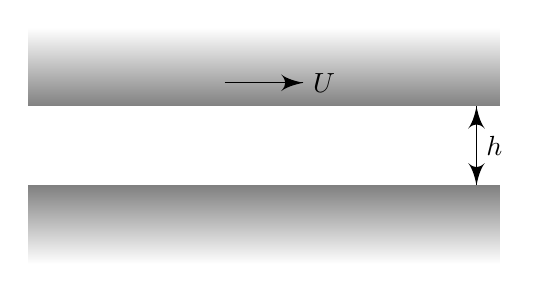
\begin{tikzpicture}
    \fill [gray, path fading=south] (0, 0) rectangle (6, -1);
    \fill [gray, path fading=north] (0, 1) rectangle (6, 2);
    \draw [->] (2.5, 1.3) -- +(1, 0) node [right] {$U$};

    \draw [<->] (5.7, 0) -- +(0, 1) node [right, pos=0.5] {$h$};
  \end{tikzpicture}
\end{center}
By definition, the stress is the force per unit area. In this case, it is the horizontal force we need to exert to keep the top plate moving.

\begin{defi}[Tangential stress]
  The \emph{tangential stress} $\tau_s$ is the force (per unit area) required to move the top plate at speed $U$.
\end{defi}
This is also the force we need to exert on the bottom plate to keep it still. Or the horizontal force at any point in fluid in order to maintain the velocity gradient.

By definition of a Newtonian fluid, this stress is proportional to the velocity gradient, i.e.
\begin{law}
  For a Newtonian fluid, we have
  \[
    \tau_s \propto \frac{U}{h}.
  \]
\end{law}

\begin{defi}[Dynamic viscosity]
  The \emph{dynamic viscosity} $\mu$ of the fluid is the constant of proportionality in
  \[
    \tau_s = \mu \frac{U}{h}.
  \]
\end{defi}

We can try to figure out the dimensions of these quantities:
\begin{align*}
  [\tau_s] &= ML^{-1} T^{-2}\\
  \left[\frac{U}{h}\right] &= T^{-1}\\
  [\mu] &= ML^{-1} T^{-1}.
\end{align*}
In SI units, $\mu$ has unit $\SI{}{\kilo\gram\per\meter\per\second}$.

We have not yet said what the fluid in the middle does. It turns out this is simple: at the bottom, the fluid is constant, and at the top, the fluid moves with velocity $U$. In between, the speed varies linearly.
\begin{center}
  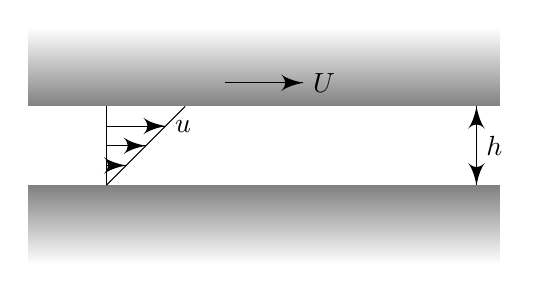
\begin{tikzpicture}
    \fill [gray, path fading=south] (0, 0) rectangle (6, -1);
    \fill [gray, path fading=north] (0, 1) rectangle (6, 2);
    \draw [->] (2.5, 1.3) -- +(1, 0) node [right] {$U$};

    \draw [<->] (5.7, 0) -- +(0, 1) node [right, pos=0.5] {$h$};

    \draw (1, 0) -- (1, 1);
    \draw (1, 0) -- (2, 1);
    \foreach \x in {0,0.25,0.5,0.75} {
      \draw [->] (1, \x) -- (1 + \x, \x);
    }
    \node at (1.75, 0.75) [right] {$u$};
  \end{tikzpicture}
\end{center}
We will derive this formally later.

For a general flow, let $u_T(\mathbf{x})$ be the velocity of the fluid at position $\mathbf{x}$. Then the velocity gradient is
\[
  \frac{\partial \mu_T(\mathbf{x})}{\partial \mathbf{n}}.
\]
Hence the tangential stress is given by
\[
  \tau_s = \mu \frac{\partial u_T(\mathbf{x})}{\partial \mathbf{n}},
\]
and is in the direction of the tangential component of velocity. Again, the normal vector $\mathbf{n}$ points \emph{into} the fluid.

\subsection{Steady parallel viscous flow}
We are first going to consider a very simple type of flow, known as \emph{steady parallel viscous flow}, and derive the equations of motion of it. We first explain what this name means. The word ``viscous'' simply means we do not assume the viscosity vanishes, and is not something new.

\begin{defi}[Steady flow]
  A \emph{steady flow} is a flow that does not change in time. In other words, all forces balance, and there is no acceleration.
\end{defi}

\begin{defi}[Parallel flow]
  A \emph{parallel flow} is a flow where the fluid only flows in one dimension (say the $x$ direction), and only depends on the direction perpendicular to a plane (say the $x-z$ plane). So the velocity can be written as
  \[
    \mathbf{u} = (u(y), 0, 0).
  \]
\end{defi}
These can be conveniently thought of as being two-dimensional, by forgetting the $z$ direction.

Note that our velocity does not depend on the $x$ direction. This can be justified by the assumption that the fluid is incompressible. If we had a velocity gradient in the $x$-direction, then we will have fluid ``piling up'' at certain places, violating incompressibility.

We will give a formal definition of incompressibility later. In general, though, fluids are not compressible. For example, sound waves are exactly waves of compression in air, and cannot exist if air is incompressible. So we can alternatively state the assumption of incompressibility as ``sound travels at infinite speed''.

Hence, compressibility matters mostly when we are travelling near the speed of sound. If we are moving in low speeds, we can just pretend the fluid is indeed incompressible. This is what we will do in this course, since the speed of sound is in general very high.

For a general steady parallel viscous flow, We can draw a flow profile like this:
\begin{center}
  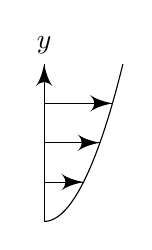
\begin{tikzpicture}
    \draw (0, 0) parabola (1, 2);
    \foreach \x in {0,0.25,0.5,0.75} {
      \pgfmathsetmacro\len{sqrt(\x)}
      \draw [->] (0, 2*\x) -- +(\len, 0);
    }
    \draw [->] (0, 0) -- (0, 2) node [above] {$y$};
  \end{tikzpicture}
\end{center}
The lengths of the arrow signify the magnitude of the velocity at that point.

To derive the equations of motion, we can consider a small box in the fluid.
\begin{center}
  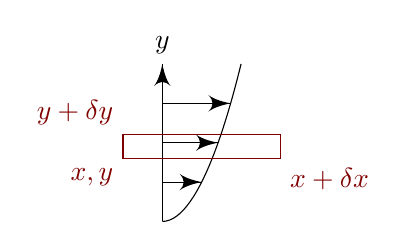
\begin{tikzpicture}
    \draw (0, 0) parabola (1, 2);
    \foreach \x in {0,0.25,0.5,0.75} {
      \pgfmathsetmacro\len{sqrt(\x)}
      \draw [->] (0, 2*\x) -- +(\len, 0);
    }
    \draw [->] (0, 0) -- (0, 2) node [above] {$y$};
    \draw [mred] (-0.5, 0.8) node [anchor = north east] {$x, y$} -- +(2, 0) node [anchor = north west] {$x + \delta x$} -- +(2, 0.3) -- +(0, 0.3) node [anchor = south east] {$y + \delta y$} -- cycle;
  \end{tikzpicture}
\end{center}
We know that this block of fluid moves in the $x$ direction without acceleration. So the total forces of the surrounding environment on the box should vanish.

We first consider the $x$ direction. There are normal stresses at the sides, and tangential stresses at the top and bottom. The sum of forces in the $x$-direction (per unit transverse width) gives
\[
  p(x) \delta y - p(x + \delta x) \delta y + \tau_s(y + \delta y) \delta x + \tau_s(y) \delta x = 0.
\]
By the definition of $\tau_s$, we can write
\[
  \tau_s(y + \delta y) = \mu \frac{\partial u}{\partial y}(y + \delta y),\quad \tau_s (y) = -\mu \frac{\partial u}{\partial y}(y),
\]
where the different signs come from the different normals (for a normal pointing downwards, $\frac{\partial}{\partial \mathbf{n}} = \frac{\partial}{\partial(-y)}$).

Dividing by $\delta x \delta y$, we get
\[
  \frac{1}{\delta x}(p(x) - p(x + \delta x)) + \mu\frac{1}{\delta y}\left(\frac{\partial u}{\partial y}(y + \delta y) - \frac{\partial u}{\partial y}(y)\right).
\]
Taking the limit as $\delta x, \delta y \to 0$, we end up with the equation of motion
\[
  -\frac{\partial p}{\partial x} + \mu \frac{\partial^2 u}{\partial y^2} = 0.
\]
Performing similar calculations in the $y$ direction, we obtain
\[
  -\frac{\partial p}{\partial y} = 0.
\]
In the second equation, we keep the negative sign for consistency, but obviously in this case it is not necessary.

This is the simplest possible case. We can extend this a bit by allowing, non-steady flows and external forces on the fluid. Then the velocity is of the form
\[
  \mathbf{u} = (u(y, t), 0, 0).
\]
Writing the external body force (per unit volume) as $(f_x, f_y, 0)$, we obtain the equations
\begin{align*}
  \rho\frac{\partial u}{\partial t} &= -\frac{\partial p}{\partial x} + \mu \frac{\partial^2 u}{\partial y^2} + f_x\\
  0 &=-\frac{\partial p}{\partial y} + f_y.
\end{align*}
The derivation of these equations is straightforward, and is left as an exercise for the reader on the example sheet. Here $\rho$ is the density, i.e.\ the mass per unit volume. For air, it is approximately $\SI{1}{\kilo\gram\per\meter\cubed}$, and for water, it is approximately $\SI{1000}{\kilo\gram\per\meter\cubed}$.

Along with equations, we also need boundary condition. In general, Newtonian fluids satisfy one of the following two boundary conditions:

\begin{enumerate}
  \item \emph{No-slip condition}: at the boundary, the tangential component of the fluid velocity equals the tangential velocity of boundary. In particular, if the boundary is stable, the tangential component of the fluid velocity is zero. This means fluids stick to surfaces.
    \[
      u_T = 0.\tag{1.5}
    \]
  \item \emph{Stress condition}: alternatively, a tangential stress $\tau$ is imposed on the fluid. In this case,
    \[
      -\mu \frac{\partial u_T}{\partial n} = \tau.
    \]
\end{enumerate}
The no-slip condition is common when we have a fluid-solid boundary, where we think the fluid ``sticks'' to the solid boundary. The stress condition is more common when we have a fluid-fluid boundary (usually liquid and gas), where we require the tangential stresses to match up. In non-parallel flow, we will often require the flow not to penetrate the solid boundary, but this is automatically satisfied in parallel flow.

We are going to look at some examples.
\begin{eg}[Couette flow]
  This is flow driven by the motion of a boundary, as we have previously seen.
  \begin{center}
    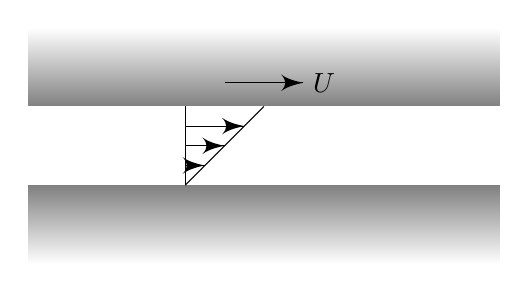
\begin{tikzpicture}
      \fill [gray, path fading=south] (0, 0) rectangle (6, -1);
      \fill [gray, path fading=north] (0, 1) rectangle (6, 2);
      \draw [->] (2.5, 1.3) -- +(1, 0) node [right] {$U$};

      \draw (2, 0) -- (2, 1);
      \draw (2, 0) -- (3, 1);

      \foreach \x in {0.25,0.5,0.75} {
        \draw [->] (2, \x) -- +(\x, 0);
      }
    \end{tikzpicture}
  \end{center}
  We assume that this is a steady flow, and there is no pressure gradient. So our equations give
  \[
    \frac{\partial^2 u}{\partial y^2} = 0.
  \]
  Moreover, the no-slip condition says $u = 0$ on $y = 0$; $u = U$ on $y = h$. The solution is thus
  \[
    u = \frac{U y}{h}.
  \]
\end{eg}

\begin{eg}[Poiseuille flow]
  This is a flow driven by a pressure gradient between stationary boundaries. Again we have two boundaries
  \begin{center}
    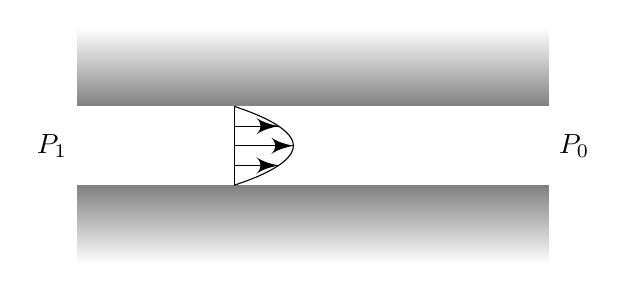
\begin{tikzpicture}
      \fill [gray, path fading=south] (0, 0) rectangle (6, -1);
      \fill [gray, path fading=north] (0, 1) rectangle (6, 2);

      \node [left] at (0, 0.5) {$P_1$};
      \node [right] at (6, 0.5) {$P_0$};

      \foreach \x in {0.25,0.5,0.75} {
        \pgfmathsetmacro\len{\x * (1 - \x)}
        \draw [->] (2, \x) -- +(3 * \len, 0);
      };
      \draw [rotate=270, yscale=-1, shift={(-3,-3)}] (2.5, 0.25) parabola (2, 1);% magic
      \draw [rotate=90, shift={(-2,-3)}] (2.5, 0.25) parabola (2, 1);
      \draw (2, 0) -- (2, 1);
    \end{tikzpicture}
  \end{center}
  We have a high pressure $P_1$ on the left, and a low pressure $P_0 < P_1$ on the right. We solve this problem again, but we will also include gravity. So the equations of motion become
  \begin{align*}
    -\frac{\partial p}{\partial x} + \mu\frac{\partial^2 u}{\partial y^2} &= 0\\
    -\frac{\partial p}{\partial y} - g\rho &= 0
  \end{align*}
  The boundary conditions are $u = 0$ at $y = 0, h$. The second equation implies
  \[
    p =- g\rho y + f(x)
  \]
  for some function $f$. Substituting into the first gives
  \[
    \mu\frac{\partial^2 u}{\partial y^2} = f'(x).
  \]
  The left is a function of $y$ only, while the right depends only on $x$. So both must be constant, say $G$. Using the boundary conditions, we get
  \[
    \mu\frac{\partial^2 u}{\partial y^2} = f'(x) = G = \frac{P_1 - P_0}{L},
  \]
  where $L$ is the length of the tube. Then we find
  \[
    u = \frac{G}{2 \mu} y(h - y).
  \]
  Here the velocity is the greatest at the middle, where $y = \frac{h}{2}$.
\end{eg}

Since the equations of motion are linear, if we have both a moving boundary and a pressure gradient, we can just add the two solutions up.

\subsection{Derived properties of a flow}
The velocity and pressure already fully describe the flow. However, there are some other useful quantities we can compute out of these.

The first thing we consider is how much stuff is being transported by the flow.
\begin{defi}[Volume flux]
  The \emph{volume flux} is the volume of fluid traversing a cross-section per unit time. This is given by
  \[
    q = \int_0^h u(y) \;\d y
  \]
  per unit transverse width.
\end{defi}
We can calculate this immediately for the two flows.

\begin{eg}
  For the Couette flow, we have
  \[
    q = \int_0^h \frac{Uy}{h}\;\d y = \frac{Uh}{2}.
  \]
  For the Poiseuille flow, we have
  \[
    q = \int_0^h \frac{G}{2\mu} y (h - y)\;\d y = \frac{Gh^3}{12 \mu}.
  \]
\end{eg}

We can also ask how much ``rotation'' there is in the flow.
\begin{defi}[Vorticity]
  The \emph{vorticity} is defined by
  \[
    \boldsymbol\omega = \nabla \times \mathbf{u}.
  \]
\end{defi}
In our case, since we have
\[
  \mathbf{u} = (u(y, t), 0, 0),
\]
we have
\[
  \boldsymbol\omega = \left(0, 0, -\frac{\partial u}{\partial y}\right).
\]
\begin{eg}
  For the case of the Couette flow, the vorticity is $\boldsymbol\omega = \left(0, 0, -\frac{U}{h}\right)$. This is a constant, i.e.\ the vorticity is uniform.
  \begin{center}
    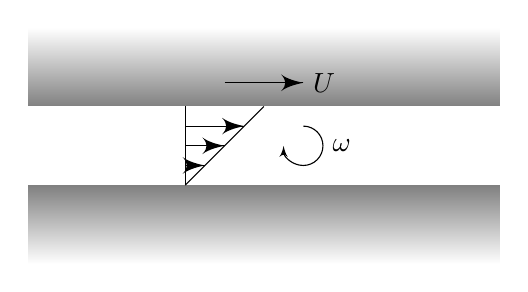
\begin{tikzpicture}
      \fill [gray, path fading=south] (0, 0) rectangle (6, -1);
      \fill [gray, path fading=north] (0, 1) rectangle (6, 2);
      \draw [->] (2.5, 1.3) -- +(1, 0) node [right] {$U$};

      \draw (2, 0) -- (2, 1);
      \draw (2, 0) -- (3, 1);

      \foreach \x in {0.25,0.5,0.75} {
        \draw [->] (2, \x) -- +(\x, 0);
      }
      \draw [-latex'] (3.5, 0.75) arc(90:-180:0.25);
      \node at (3.75, 0.5) [right] {$\omega$};
    \end{tikzpicture}
  \end{center}
  For the case of the Poiseuille flow, we have
  \[
    \boldsymbol\omega = \left(0, 0, \frac{G}{\mu}\left(y - \frac{h}{2}\right)\right).
  \]
  \begin{center}
    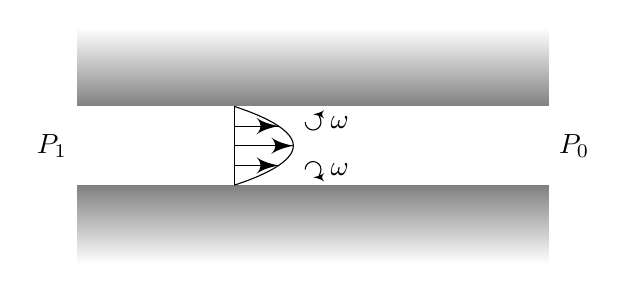
\begin{tikzpicture}
      \fill [gray, path fading=south] (0, 0) rectangle (6, -1);
      \fill [gray, path fading=north] (0, 1) rectangle (6, 2);

      \node [left] at (0, 0.5) {$P_1$};
      \node [right] at (6, 0.5) {$P_0$};

      \foreach \x in {0.25,0.5,0.75} {
        \pgfmathsetmacro\len{\x * (1 - \x)}
        \draw [->] (2, \x) -- +(3 * \len, 0);
      };
      \draw [rotate=270, yscale=-1, shift={(-3,-3)}] (2.5, 0.25) parabola (2, 1);% magic
      \draw [rotate=90, shift={(-2,-3)}] (2.5, 0.25) parabola (2, 1);
      \draw (2, 0) -- (2, 1);

      \draw [-latex'] (2.9, 0.2) arc(180:-90:0.1);
      \node at (3.1, 0.2) [right] {$\omega$};

      \draw [-latex'] (2.9, 0.8) arc(-180:90:0.1);
      \node at (3.1, 0.8) [right] {$\omega$};
    \end{tikzpicture}
  \end{center}
\end{eg}

Recall that the tangential stress $\tau_s$ is the tangential force per unit area exerted by the fluid on the surface, given by
\[
  \tau_s = \mu \frac{\partial u}{\partial \mathbf{n}},
\]
with $\mathbf{n}$ pointing into the fluid.

\begin{eg}
  For the Couette flow, we have
  \[
    \tau_s =
    \begin{cases}
      \mu \frac{U}{h} & y = 0\\
      -\mu \frac{U}{h} & y = h
    \end{cases}.
  \]
  We see that at $y = 0$, the stress is positive, and pulls the surface forward. At $y = h$, it is negative, and the surface is pulled backwards.

  For the Poiseuille flow, we have
  \[
    \tau_s =
    \begin{cases}
      \frac{Gh}{2} & y = 0\\
      \frac{Gh}{2} & y = h\\
    \end{cases}
  \]
  Both surfaces are pulled forward, and this is independent of the viscosity. This makes sense since the force on the surface is given by the pressure gradient, which is independent of the fluid.
\end{eg}

\subsection{More examples}
Since we are probably bored by the Couette and Poiseuille flows, we do another more interesting example.
\begin{eg}[Gravity-driven flow down a slope]
  Suppose we have some fluid flowing along a slope.
  \begin{center}
    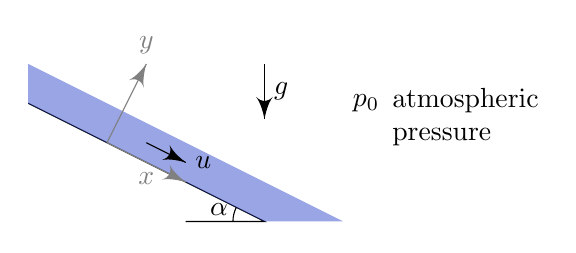
\begin{tikzpicture}
      \draw (0, 1.5) -- (3, 0) -- (2, 0);
      \fill [mblue, opacity=0.5] (0, 1.5) -- (3, 0) -- (4, 0) -- (0, 2) -- cycle;

      \draw [gray, ->] (1, 1) -- +(0.5, 1) node [above] {$y$};
      \draw [gray, ->] (1, 1) -- +(1, -0.5) node [below, pos=0.5] {$x$};
      \draw [->] (3, 2) -- +(0, -0.7) node [pos=0.5, right] {$g$};
      \draw [->] (1.5, 1) -- (2, 0.75) node [right] {$u$};
      \node [right] at (4, 1.5) {$p_0$};
      \node [right, align=left] at (4.5, 1.33) {atmospheric\\ pressure};
      \draw (2.6, 0) arc(180:153.4349:0.4);
      \node [left] at (2.66, 0.15) {$\alpha$};
    \end{tikzpicture}
  \end{center}
  Here there is just atmosphere above the fluid, and we assume the fluid flow is steady, i.e.\ $u$ is merely a function of $y$. We further assume that the atmospheric pressure does not vary over the vertical extent of the flow. This is a very good approximation because $\rho_{\mathrm{air}} \ll \rho_{\mathrm{liq}}$.

  Similarly, we assume $\mu_{\mathrm{air}} \ll \mu_{\mathrm{liq}}$. So the air exerts no significant tangential stress. This is known as a free surface.

  We first solve the $y$ momentum equation. The force in the $y$ direction is $-g \rho \cos \alpha$. Hence the equation is
  \[
    \frac{\partial p}{\partial y} = - gp \cos \alpha.
  \]
  Using the fact that $p = p_0$ at the top boundary, we get
  \[
    p = p_0 - g\rho \cos \alpha (y - h).
  \]
  In particular, $p$ is independent of $x$. In the $x$ component, we get
  \[
    \mu \frac{\partial^2 u}{\partial y^2} = - g\rho \sin \alpha.
  \]
  The no slip condition gives $u = 0$ when $y = 0$. The other condition is that there is no stress at $y = h$. So we get $\frac{\partial u}{\partial y} = 0$ when $y = h$.

  The solution is thus
  \[
    u = \frac{g\rho\sin \alpha}{2 \mu} y(2h - y).
  \]
  This is a bit like the Poiseuille flow, with $\frac{gp \sin \alpha}{2\mu}$ as the pressure gradient. But instead of going to zero at $y = h$, we get to zero at $y = 2h$ instead. So this is half a Poiseuille flow. % diagram

  It is an exercise for the reader to calculate the volume flux $q$.
\end{eg}

For a change, we do a case where we have \emph{unsteady} flow.
\begin{eg}
  Consider fluid initially at rest in $y > 0$, resting on a flat surface.
  \begin{center}
    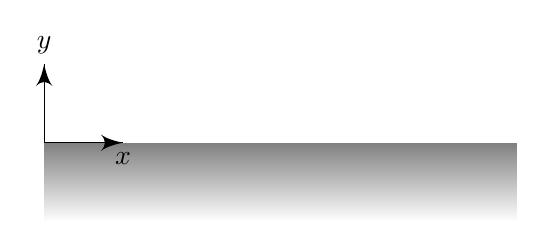
\begin{tikzpicture}
      \fill [gray, path fading=south] (0, 0) rectangle (6, -1);
      \draw [->] (0, 0) -- (0, 1) node [above] {$y$};
      \draw [->] (0, 0) -- (1 , 0) node [below] {$x$};
    \end{tikzpicture}
  \end{center}
  At time $t = 0$, the boundary $y = 0$ starts to move at constant speed $U$. There is no force and no pressure gradient.

  We use the $x$-momentum equation to get
  \[
    \frac{\partial u}{\partial t} = \nu \frac{\partial^2 u}{\partial y^2},
  \]
  where $\nu = \frac{\mu}{\rho}$. This is clearly the diffusion equation, with the diffusivity $\nu$. We can view this as the diffusion coefficient for motion/momentum/vorticity.
  \begin{defi}[Kinematic viscosity]
    The \emph{kinematic viscosity} is
    \[
      \nu = \frac{\mu}{\rho}.
    \]
  \end{defi}
  The boundary conditions are $u = 0$ for $t = 0$ and $u \to 0$ as $y \to \infty$ for all $t$. The other boundary condition is obviously $u = U$ when $y = 0$, for $t > 0$.

  You should have learnt how to solve this in, say, IB Methods. We will approach this differently here.

  Before we start, we try to do some dimensional analysis, and try to figure out how far we have to go away from the boundary before we don't feel any significant motion.

  We first list all the terms involved. We are already provided with a velocity $U$. We let $T$ be our time scale. We would like to know how fast the movement of fluid propagates up the $y$ axis. We note that in this case, we don't really have an extrinsic length scale --- in the case where we have two boundaries, the distance between them is a natural length scale to compare with, but here the fluid is infinitely thick. So we need to come up with a characteristic intrinsic length scale somewhat arbitrarily. For example, at any time $T$, we can let $\delta$ be the amount of fluid that has reached a speed of at least $\frac{U}{10}$ (that was completely arbitrary).

  Instead of trying to figure out the dimensions of, say, $\nu$ and trying to match them, we just replace terms in the differential equation with these quantities of the right dimension, since we know our differential equation is dimensionally correct. So we obtain
  \[
    \frac{U}{T} \sim \nu \frac{U}{\delta^2}.
  \]
  Since the $U$ cancels out, we get
  \[
    \delta \sim \sqrt{\nu T}.
  \]
  We can figure out approximately how big this is, using the table below:
  \begin{center}
    \begin{tabular}{cccc}
      \toprule
      & $\mu(\SI{}{\kilo\gram\per\meter\per\second})$ & $\rho(\SI{}{\kilo\gram\per\meter\cubed})$ & $\nu(\SI{}{\meter\squared\per\second})$\\
      \midrule
      water & $10^{-3}$ & $10^3$ & $10^{-6}$\\
      air & $10^{-5}$ & $1$ & $10^{-5}$\\
      \bottomrule
    \end{tabular}
  \end{center}
  These are, in general, very tiny. So we expect to feel nothing when we move slightly away from the boundary.

  We now solve the problem properly. In an infinite domain with no extrinsic length scale, the diffusion equation admits a similarity solution. We write
  \[
    u(y, t) = U f(\eta),
  \]
  where $f(\eta)$ is a dimensionless function of the dimensionless variable $\eta$. To turn $y$ into a dimensionless variable, we have to define
  \[
    \eta = \frac{y}{\delta} = \frac{y}{\sqrt{\nu t}}.
  \]
  We substitute this form of the solution into the differential equation. Then we get
  \[
    -\frac{1}{2} \eta f'(\eta) = f''(\eta),
  \]
  with boundary condition $f = 1$ on $\eta = 0$. Then the solution is by definition
  \[
    f = \erfc \left(\frac{\eta}{2}\right).
  \]
  Hence
  \[
    u = U \erfc \left(\frac{y}{2\sqrt{\eta t}}\right).
  \]
  \begin{center}
    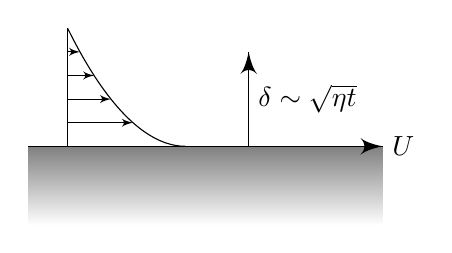
\begin{tikzpicture}
      \fill [gray, path fading=south] (0.5, 0) rectangle (5, -1);
      \draw [->] (0.5, 0) -- (5, 0) node [right] {$U$};
      \draw [->] (3.3, 0) -- +(0, 1.2) node [right, pos=0.5] {$\delta \sim \sqrt{\eta t}$};

      \draw (1, 0) -- (1, 1.5);
      \draw (2.5, 0) parabola (1, 1.5);
      \foreach \y in {0.3,0.6,0.9,1.2} {
        \pgfmathsetmacro\x{1.5 - sqrt(1.5 * \y)};
        \draw [-latex'] (1, \y) -- +(\x, 0);
      }
    \end{tikzpicture}
  \end{center}
  We can compute the tangential stress of the fluid in the above case to be
  \[
    \tau_s = \mu\frac{\partial u}{\partial y} = \left.\mu \frac{U}{\sqrt{\nu t}} \left(\frac{2}{\sqrt{\pi}}\right) e^{-y^{2}}\right|_{y = 0} = \frac{\mu U}{\sqrt{\pi \nu t}}.
  \]
  Using our previous calculations of the kinematic viscosities, we find that $\frac{\mu}{\sqrt{\nu}}$ is $1$ for water and $10^{-3}$ for air.

  This is significant in, say, the motion of ocean current. When the wind blows, it causes the water in the ocean to move along with it. This is done in a way such that the surface tension between the two fluids match at the boundary. Hence we see that even if the air blows really quickly, the resultant ocean current is much smaller, say a hundredth to a thousandth of it.
\end{eg}

\section{Kinematics}
So far, we have considered a rather specific kind of fluid flow --- parallel flow, and derived the equations of motion from first principles. From now on, we will start to consider more general theory of fluid dynamics. In this section, we are mostly making some definitions and descriptions of flows. In the next chapter, we will take the equations of motion and try to solve them in certain scenarios.

\subsection{Material time derivative}
We first want to consider the problem of how we can measure the change in a quantity, say $f$. This might be pressure, velocity, temperature, or anything else you can imagine.

The obvious thing to do would be the consider the time derivative
\[
  \frac{\partial f}{\partial t}.
\]
In physical terms, this would be equivalent to fixing our measurement instrument at a point and measure the quantity over time. This is known as the \emph{Eulerian picture}.

However, often we want to consider something else. We pretend we are a fluid particle, and move along with the flow. We then measure the change in $f$ along our trajectory. This is known as the \emph{Lagrangian picture}.

Let's look at these two pictures, and see how they relate to each other. Consider a time-dependent field $f(\mathbf{x}, t)$. For example, it might be the pressure of the system, or the temperature of the fluid. Consider a path $\mathbf{x}(t)$ through the field, and we want to know how the field varies as we move along the path.

Along the path $\mathbf{x}(t)$, the chain rule gives
\begin{align*}
  \frac{\d f}{\d t}(\mathbf{x}(t), t) &= \frac{\partial f}{\partial x} \frac{\d x}{\d t} + \frac{\partial f}{\partial y}\frac{\d y}{\d t} + \frac{\partial f}{\partial z}\frac{\d z}{\d t} + \frac{\partial f}{\partial t}\\
  &= \nabla f \cdot \dot{\mathbf{x}} + \frac{\partial f}{\partial t}.
\end{align*}
\begin{defi}[Material derivative]
  If $\mathbf{x}(t)$ is the (Lagrangian) path followed by a fluid particle, then necessarily $\dot{\mathbf{x}}(t) = \mathbf{u}$ by definition. In this case, we write
  \[
    \frac{\d f}{\d t} = \frac{\D f}{\D t}.
  \]
  This is the \emph{material derivative}.

  In other words, we have
  \[
    \frac{\D f}{\D t} = \mathbf{u}\cdot \nabla f + \frac{\partial f}{\partial t}.
  \]
\end{defi}
On the left of this equation, we have the \emph{Lagrangian derivative}, which is the change in $f$ as we follow the path. On the right of this equation, the first term is the \emph{advective derivative}, which is the change due to change in position. The second term is $\frac{\partial f}{\partial t}$, the \emph{Eulerian time derivative}, which is the change at a fixed point.

For example, consider a river that gets wider as we go downstream. We know (from, say, experience) that the flow is faster upstream than downstream. If the motion is steady, then the Eulerian time derivative vanishes, but the Lagrangian derivative does not, since as the fluid goes down the stream, the fluid slows down, and there is a spacial variation.

Often, it is the Lagrangian derivative that is relevant, but the Eulerian time derivative is what we can usually put into differential equations. So we will need both of them, and relate them by the formula above.

\subsection{Conservation of mass}
We can start formulating equations. The first one is the conservation of mass.

We fix an arbitrary region of space $\mathcal{D}$ with boundary $\partial \mathcal{D}$ and outward normal $\mathbf{n}$. We imagine there is some flow through this volume
\begin{center}
  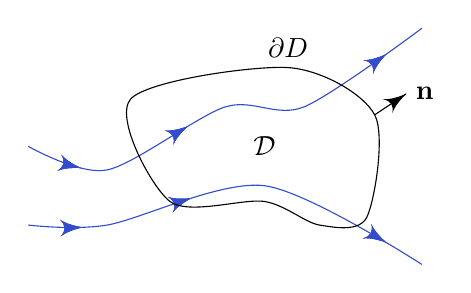
\begin{tikzpicture}
    \draw [mblue, ->-=0.13, ->-=0.4, ->-=0.9] plot [smooth] coordinates {(-3, 0) (-2, -0.3) (-0.5, 0.5) (0.5, 0.5) (2, 1.5)};
    \draw [mblue, ->-=0.13, ->-=0.4, ->-=0.9] plot [smooth] coordinates {(-3, -1) (-2, -1) (0, -0.5) (2, -1.5)};
    \draw plot [smooth cycle] coordinates {(-1.2, -0.7) (0, -0.7) (0.7, -1) (1.3, -0.9) (1.4, 0.4) (0.3, 1) (-1.7, 0.6)};
    \node at (0, 0) {$\mathcal{D}$};
    \node [above] at (0.3, 1) {$\partial D$};
    \draw [->] (1.4, 0.4) -- +(0.4, 0.2666) node [right] {$\mathbf{n}$};
  \end{tikzpicture}
\end{center}
What we want to say is that the change in the mass inside $\mathcal{D}$ is equal to the total flow of fluid through the boundary. We can write this as
\[
  \frac{\d }{\d t}\int_{\mathcal{D}} \rho \;\d V = -\int_{\partial \mathcal{D}} \rho \mathbf{u}\cdot \mathbf{n}\;\d S.
\]
We have the negative sign since we picked the outward normal, and hence the integral measures the outward flow of fluid.

Since the domain is fixed, we can interchange the derivative and the integral on the left; on the right, we can use the divergence theorem to get
\[
  \int_{\mathcal{D}} \left(\frac{\partial \rho}{\partial t} + \nabla \cdot (\rho \mathbf{u})\right) \;\d V = 0.
\]
Since $\mathcal{D}$ was arbitrary, we must have
\[
  \frac{\partial \rho}{\partial t} + \nabla \cdot (\rho \mathbf{u}) = 0
\]
everywhere in space.

This is the general form of a conservation law --- the rate of change of ``stuff'' density plus the divergence of the ``stuff flux'' is constantly zero. Similar conservation laws appear everywhere in physics.

In the conservation equation, we can expand $\nabla \cdot (\rho \mathbf{u})$ to get
\[
  \frac{\partial \rho}{\partial t} + \mathbf{u}\cdot \nabla \rho + \rho \nabla \cdot \mathbf{u} = 0.
\]
We notice the first term is just the material derivative of $\rho$. So we get
\[
  \frac{\D \rho}{\D t} + \rho \nabla \cdot \mathbf{u} = 0.
\]
With the conservation of mass, we can now properly say what incompressibility is. What exactly happens when we compress a fluid? When we compress mass, in order to conserve mass, we must increase the density. If we don't allow changes in density, then the material derivative $\frac{\D \rho}{\D t}$ must vanish. So we define an incompressible fluid as follows:
\begin{defi}[Incompressible fluid]
  A fluid is \emph{incompressible} if the density of a fluid particle does not change. This implies
  \[
    \frac{\D \rho}{\D t} = 0,
  \]
  and hence
  \[
    \nabla \cdot \mathbf{u} = 0.
  \]
  This is also known as the \emph{continuity equation}.
\end{defi}
For parallel flow, $\mathbf{u} = (u, 0, 0)$. So if the flow is incompressible, we must have $\frac{\partial u}{\partial x} = \nabla \cdot \mathbf{u} = 0$. So we considered $u$ of the form $u = u(y, z, t)$.

Of course, incompressibility is just an approximation. Since we can hear things, everything must be compressible. So what really matters is whether the slow speed is small compared to the speed of sound. If it is relatively small, then incompressibility is a good approximation. In air, the speed of sound is approximately $\SI{340}{\meter\per\second}$. In water, the speed of sound is approximately $\SI{1500}{\meter\per\second}$.

\subsection{Kinematic boundary conditions}
Suppose our system has a boundary. There are two possible cases --- either the boundary is rigid, like a wall, or it moves with the fluid. In either case, fluids are not allowed to pass through the boundary.

To deal with boundaries, we first suppose it has a velocity $\mathbf{U}$ (which may vary with position if the boundary extends through space). We define a local reference frame moving with velocity $\mathbf{U}$, so that in this frame of reference, the boundary is stationary.

In this frame of reference, the fluid has relative velocity
\[
  \mathbf{u}' = \mathbf{u} - \mathbf{U}.
\]
As we mentioned, fluids are not allowed to cross the boundary. Let the normal to the boundary be $\mathbf{n}$, then we must have
\[
  \mathbf{u}' \cdot \mathbf{n} = 0.
\]
In terms of the outside frame, we get
\[
  \mathbf{u}\cdot \mathbf{n} = \mathbf{U} \cdot \mathbf{n}.
\]
This is the condition we have for the boundary.

If we have a stationary rigid boundary, e.g.\ the wall, then $\mathbf{U} = \mathbf{0}$. So our boundary condition is
\[
  \mathbf{u}\cdot \mathbf{n}= 0.
\]
Free boundaries are more complicated. A good example of a free material boundary is the surface of a water wave, or interface between two immiscible fluids --- say oil and water.
\begin{center}
  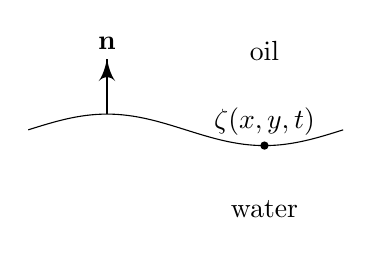
\begin{tikzpicture}
    \draw (0, 0) sin (1, 0.2) cos (2, 0) sin (3, -0.2) cos (4, 0);
    \node at (3, 1) {oil};
    \node at (3, -1) {water};

    \draw [->] (1, 0.2) -- +(0, 0.7) node [above] {$\mathbf{n}$};

    \node [circ] at (3, -0.2) {};
    \node [above] at (3, -0.2) {$\zeta(x, y, t)$};
  \end{tikzpicture}
\end{center}
We can define the surface by a function
\[
  z = \zeta(x, y, t).
\]
We can alternatively define the surface as a contour of
\[
  F(x, y, z, t) = z - \zeta(x, y, t).
\]
Then the surface is defined by $F = 0$. By IA Vector Calculus, the normal is parallel to
\[
  \mathbf{n} \parallel \nabla F = (-\zeta_x, -\zeta_y, 1).
\]
Also, we have
\[
  \mathbf{U} = (0, 0, \zeta_t).
\]
We now let the velocity of the fluid be
\[
  \mathbf{u} = (u, v, w).
\]
Then the boundary condition requires
\[
  \mathbf{u}\cdot \mathbf{n} = \mathbf{U}\cdot \mathbf{n}.
\]
In other words, we have
\[
  -u \zeta_x - v\zeta_y + w = \zeta_t.
\]
So we get
\[
  w = u \zeta_x + v\zeta_y + \zeta_t = \mathbf{u}\cdot \nabla \zeta + \frac{\partial \zeta}{\partial t} = \frac{\D \zeta}{\D t}.
\]
So all the boundary condition says is
\[
  \frac{\D \zeta}{\D t} = w.
\]
Alternatively, since $F$ is a material surface, its material derivative must vanish. So
\[
  \frac{\D F}{\D t} = 0,
\]
and this just gives the same result as above. We will discuss surface waves towards the end of the course, and then come back and use this condition.

\subsection{Streamfunction for incompressible flow}
We suppose our fluid is incompressible, i.e.
\[
  \nabla \cdot \mathbf{u} = 0.
\]
By IA Vector Calculus, this implies there is a vector potential $\mathbf{A}$ such that
\begin{defi}[Vector potential]
  A \emph{vector potential} is an $\mathbf{A}$ such that
  \[
    \mathbf{u} = \nabla \times \mathbf{A}.
  \]
\end{defi}

In the special case where the flow is two dimensional, say
\[
  \mathbf{u} = (u(x, y, t), v(x, y, t), 0),
\]
we can immediately know $\mathbf{A}$ is of the form
\[
  \mathbf{A} = (0, 0, \psi(x, y, t)),
\]
Taking the curl of this, we get
\[
  \mathbf{u} = \left(\frac{\partial \psi}{\partial y}, -\frac{\partial \psi}{\partial x}, 0\right).
\]
\begin{defi}[Streamfunction]
  The $\psi$ such that $\mathbf{A} = (0, 0, \psi)$ is the \emph{streamfunction}.
\end{defi}
This streamfunction is both physically significant, and mathematically convenient, as we will soon see.

We look at some properties of the streamfunction. The first thing we can do is to look at the contours $\psi = c$. These have normal
\[
  \mathbf{n} = \nabla \psi = \left(\psi_x, \psi_y, 0\right).
\]
We immediately see that
\[
  \mathbf{u}\cdot \mathbf{n} = \frac{\partial \psi}{\partial x} \frac{\partial \psi}{\partial y} - \frac{\partial \psi}{\partial y}\frac{\partial \psi}{\partial x} = 0.
\]
So the flow is perpendicular to the normal, i.e.\ tangent to the contours of $\psi$.
\begin{defi}[Streamlines]
  The \emph{streamlines} are the contours of the streamfunction $\psi$.
\end{defi}
This gives an instantaneous picture of flow.

Note that if the flow is \emph{unsteady}, then the streamlines are \emph{not} particle paths.
\begin{eg}
  Consider $\mathbf{u} = (t, 1, 0)$. When $t = 0$, the velocity is purely in the $y$ direction, and the streamlines are also vertical; at $t = 1$, the velocity makes an $45^\circ$ angle with the horizontal, and the streamlines are slanted:
  \begin{center}
    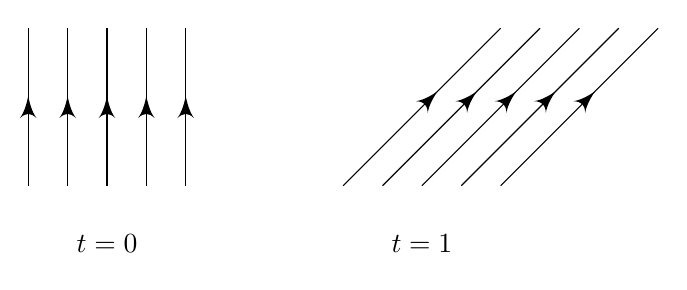
\begin{tikzpicture}
      \draw [->-=0.57] (0, 0) -- +(0, 2);
      \draw [->-=0.57] (0.5, 0) -- +(0, 2);
      \draw [->-=0.57] (1, 0) -- +(0, 2);
      \draw [->-=0.57] (1.5, 0) -- +(0, 2);
      \draw [->-=0.57] (2, 0) -- +(0, 2);

      \node [below] at (1, -0.5) {$t = 0$};

      \begin{scope}[shift={(4, 0)}]
        \draw [->-=0.6] (0, 0) -- +(2, 2);
        \draw [->-=0.6] (0.5, 0) -- +(2, 2);
        \draw [->-=0.6] (1, 0) -- +(2, 2);
        \draw [->-=0.6] (1.5, 0) -- +(2, 2);
        \draw [->-=0.6] (2, 0) -- +(2, 2);

        \node [below] at (1, -0.5) {$t = 1$};
      \end{scope}
    \end{tikzpicture}
  \end{center}
  However, \emph{no} particles will actually follow any of these streamlines. For a particle released at $\mathbf{x}_0 = (x_0, y_0)$. Then we get
  \[
    \dot{x}(t) = u = t,\quad \dot{y} = v = 1.
  \]
  Hence we get
  \[
    x = \frac{1}{2}t^2 + x_0,\quad y = t + y_0.
  \]
  Eliminating $t$, we get that the path is given by
  \[
    (x - x_0) = \frac{1}{2}(y - y_0)^2.
  \]
  So the particle paths are parabolas.
\end{eg}
Typically, we draw streamlines that are ``evenly spaced'', i.e.\ we pick the streamlines $\psi = c_0$, $\psi = c_1$, $\psi = c_2$ etc. such that $c_3 - c_2 = c_2 - c_1$.

Then we know the flow is faster where streamlines are closer together:
\begin{center}
  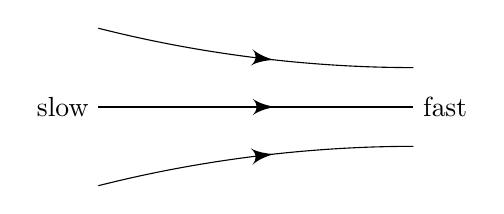
\begin{tikzpicture}
    \draw [-<-=0.44] (4, 0.5) parabola (0, 1);
    \draw [-<-=0.44] (4, 0) -- (0, 0);
    \draw [-<-=0.44] (4, -0.5) parabola (0, -1);

    \node [left] {slow};
    \node [right] at (4, 0) {fast};
  \end{tikzpicture}
\end{center}
This is since the fluid between any two stream lines must be between the stream lines. So if the flow is incompressible, to conserve mass, they mast move faster when the streamlines are closer.

We can also consider the volume flux (per unit length in the $z$-direction), crossing any curve from $\mathbf{x}_0$ to $\mathbf{x}_1$.
\begin{center}
  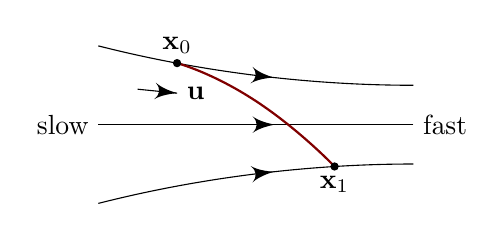
\begin{tikzpicture}
    \draw [-<-=0.44] (4, 0.5) parabola (0, 1);
    \draw [-<-=0.44] (4, 0) -- (0, 0);
    \draw [-<-=0.44] (4, -0.5) parabola (0, -1);

    \draw [mred, thick] plot [smooth, tension=1] coordinates {(1, 0.78125) (2, 0.3) (3, -0.53125)};
    \node [left] {slow};
    \node [right] at (4, 0) {fast};

    \node [circ] at (1, 0.78125) {};
    \node [above] at (1, 0.78125) {$\mathbf{x}_0$};
    \node [circ] at (3, -0.53125) {};
    \node [below] at (3, -0.53125) {$\mathbf{x}_1$};

    \draw [->] (0.5, 0.45) -- (1, 0.4) node [right] {$\mathbf{u}$};

  \end{tikzpicture}
\end{center}
Then the volume flux is
\[
  q = \int_{\mathbf{x}_0}^{\mathbf{x}_1} \mathbf{u}\cdot \mathbf{n}\;\d \ell.
\]
We see that
\[
  \mathbf{n}\;\d \ell = (-\d y, \d x).
\]
So we can write this as
\[
  q = \int_{\mathbf{x}_0}^{\mathbf{x}_1} -\frac{\partial \psi}{\partial y}\;\d y - \frac{\partial \psi}{\partial x}\;\d x = \psi(\mathbf{x}_0) - \psi(\mathbf{x}_1).
\]
So the flux depends only the difference in the value of $\psi$. Hence, for closer streamlines, to maintain the same volume flux, we need a higher speed.

Also, note that $\psi$ is constant on a stationary rigid boundary, i.e.\ the boundary is a streamline, since the flow is tangential at the boundary. This is a consequence of $\mathbf{u}\cdot \mathbf{n} = 0$. We often choose $\psi = 0$ as our boundary.

Sometimes it is convenient to consider the case when we have plane polars. We embed these in cylindrical polars $(r, \theta, z)$. Then we have
\[
  \mathbf{u} = \nabla \times (0, 0, \psi) = \frac{1}{r}
  \begin{vmatrix}
    \mathbf{e}_r & r \mathbf{e}_\theta & \mathbf{e}_z\\
    \partial_r & \partial_\theta & \partial_z\\
    0 & 0 & \psi
  \end{vmatrix}
  =\left(r \frac{\partial \psi}{\partial \theta}, -\frac{\partial \psi}{\partial r}, 0\right).
\]
As an exercise, we can verify that $\nabla \cdot \mathbf{u} = 0$. It is convenient to note that in plane polars,
\[
  \nabla \cdot \mathbf{u} = \frac{1}{r} \frac{\partial}{\partial r} (r \mathbf{u}_r) + \frac{1}{r} \frac{\partial u_\theta}{\partial \theta}.
\]

\section{Dynamics}
\subsection{Navier-Stokes equations}
So far, we haven't done anything useful. We have not yet come up with an equation of motion for fluids, and thus we don't know how fluids actually behave. The equations for the parallel viscous flow was a good start, and it turns out the general equation of motion is of a rather similar form.

Unfortunately, the equation is rather complicated and difficult to derive, and we will not derive it in this course. Instead, it is left for the Part II course. However, we will be able to derive some special cases of it later under certain simplifying assumptions.
\begin{law}[Navier-Stokes equation]
  \[
    \rho \frac{\D \mathbf{u}}{\D t} = - \nabla p + \mu \nabla^2 \mathbf{u} + \mathbf{f}.
  \]
\end{law}
This is the general equation for fluid motion. The left hand side is mass times acceleration, and the right is the individual forces --- the pressure gradient, viscosity, and the body forces (per unit volume) respectively.

In general, these are very difficult equations to solve because of non-linearity. For example, in the material derivative, we have the term $\mathbf{u} \cdot \nabla \mathbf{u}$.

There are a few things to note:
\begin{enumerate}
  \item The acceleration of a fluid particle is the Lagrangian material derivative of the velocity.
  \item The derivation of the viscous term is complicated, since for each side of the cube, there is one normal direction and two tangential directions. Thus this requires consideration of the \emph{stress tensor}. This is only done in IID Fluid Dynamics.
  \item In a gravitational field, we just have $\mathbf{f} = \mathbf{g}\rho$. This is the only body force we will consider in this course.
  \item Note that $\nabla^2 \mathbf{u}$ can be written as
    \[
      \nabla^2 \mathbf{u} = \nabla (\nabla \cdot \mathbf{u}) - \nabla \times (\nabla \times \mathbf{u}).
    \]
    In an incompressible fluid, this reduces to
    \[
      \nabla^2 \mathbf{u} = -\nabla \times (\nabla \times \mathbf{u}) = -\nabla \times \boldsymbol\omega,
    \]
    where $\boldsymbol\omega = \nabla \times \mathbf{u}$ is the vorticity. In Cartesian coordinates, for $\mathbf{u} = (u_x, u_y, u_z)$, we have
    \[
      \nabla^2 \mathbf{u} = (\nabla^2 u_x, \nabla^2 u_y, \nabla^2 u_z),
    \]
    where
    \[
      \nabla^2 = \pd[2]{x} + \pd[2]{y} + \pd[2]{z}.
    \]
  \item The Navier-Stokes equation reduces to the parallel flow equation in the special case of parallel flow, i.e.\ $\mathbf{u} = (u(y, t), 0, 0)$. This verification is left as an exercise for the reader.
\end{enumerate}

\subsection{Pressure}
In the Navier-Stokes equation, we have a pressure term. In general, we classify the pressure into two categories. If there is gravity, then we will get pressure in the fluid due to the weight of fluid above it. This is what we call \emph{hydrostatic pressure}. Technically, this is the pressure in a fluid at rest, i.e.\ when $\mathbf{u} = \mathbf{0}$.

We denote the hydrostatic pressure as $p_H$. To find this, we put in $\mathbf{u} = 0$ into the Navier-Stokes equation to get
\[
  \nabla p_H = \mathbf{f} = \rho \mathbf{g}.
\]
We can integrate this to obtain
\[
  p_H = p \mathbf{g}\cdot \mathbf{x} + p_0,
\]
where $p_0$ is some arbitrary constant. Usually, we have $\mathbf{g} = (0, 0, -g)$. Then
\[
  p_H = p_0 - g \rho z.
\]
This exactly says that the hydrostatic pressure is the weight of the fluid above you.

What can we infer from this? Suppose we have a body $\mathcal{D}$ with boundary $\partial \mathcal{D}$ and outward normal $\mathbf{n}$. Then the force due to the pressure is
\begin{align*}
  \mathbf{F} &= - \int_{\partial \mathcal{D}} p_H \mathbf{n}\cdot dS \\
  &= - \int_\mathcal{D} \nabla p_H \;\d V\\
  &= - \int_{\mathcal{D}} \mathbf{g} \rho \;\d V\\
  &= - \mathbf{g} \int_\mathcal{D} \rho \;\d V\\
  &= - M\mathbf{g},
\end{align*}
where $M$ is the mass of fluid displaced. This is known as \emph{Archimedes' principle}.

In particular, if the body is less dense than the fluid, it will float; if the body is denser than the fluid, it will sink; if the density is the same, then it does not move, and we say it is neutrally buoyant.

This is valid only when nothing is moving, since that was our assumption. Things can be very different when things are moving, which is why planes can fly.

In general, when there is motion, we might expect some other pressure gradient. It can either be some external pressure gradient driving the motion (e.g.\ in the case of Poiseuille flow), or a pressure gradient caused by the flow itself. In either case, we can write
\[
  p = p_H + p',
\]
where $p_H$ is the hydrostatic pressure, and $p'$ is what caused/results from motion.

We substitute this into the Navier-Stokes equation to obtain
\[
  \rho \frac{\D u}{\D t} = -\nabla p' + \mu \nabla^2 \mathbf{u}.
\]
So the hydrostatic pressure term cancels with the gravitational term. What we usually do is drop the ``prime'', and just look at the deviation from hydrostatic pressure. What this means is that gravity no longer plays a role, and we can ignore gravity in any flow in which the density is constant. Then all fluid particles are neutrally buoyant. This is the case in most of the course, except when we consider motion of water waves, since there is a difference in air density and water density.

\subsection{Reynolds number}
As we mentioned, the Navier-Stokes equation is very difficult to solve. So we want to find some approximations to the equation. We would like to know if we can ignore some terms. For example, if we can neglect the viscous term, then we are left with a first-order equation, not a second-order one.

To do so, we look at the balance of terms, and see if some terms dominate the others. This is done via Reynolds number.

We suppose the flow has a characteristic speed $U$ and an extrinsic length scale $L$, externally imposed by geometry. For example, if we look at the flow between two planes, the characteristic speed can be the maximum (or average) speed of the fluid, and a sensible length scale would be the length between the planes.

Next, we have to define the time scale $T = L/U$. Finally, we suppose pressure \emph{differences} have characteristic magnitude $P$. We are concerned with differences since it is pressure differences that drive the flow.

We are going to take the Navier-Stokes equation, and look at the scales of the terms. Dividing by $\rho$, we get
\begin{alignat*}{4}
  \frac{\partial \mathbf{u}}{\partial t} &{}+{}& \mathbf{u}\cdot \nabla \mathbf{u} &{}={}& -\frac{1}{\rho} \nabla p &{}+{}& \nu \nabla^2 \mathbf{u},\\
  \intertext{where again $\nu = \frac{\mu}{\rho}$. We are going to estimate the size of these terms. We get}
  \frac{U}{(L/U)} &&U \cdot \frac{U}{L} &&\frac{1}{\rho} \frac{P}{L} &&\nu \frac{U}{L^2}.
  \intertext{Dividing by $U^2/L$, we get}
  1 && 1 && \frac{P}{\rho U^2} && \frac{\nu}{UL}.
\end{alignat*}
\begin{defi}[Reynolds number]
  The \emph{Reynolds number} is
  \[
    Re = \frac{UL}{\nu},
  \]
  which is a dimensionless number. This is a measure of the magnitude of the inertia to viscous terms.
\end{defi}
So if $Re$ is very large, then the viscous term is small, and we can probably neglect it. For example, for an aircraft, we have $U \sim 10^4$, $L \sim 10$ and $\nu \sim 10^{-5}$. So the Reynolds number is large, and we can ignore the viscous term. On the other hand, if we have a small slow-moving object in viscous fluid, then $Re$ will be small, and the viscous term is significant.

Note that the pressure always scales to balance the dominant terms in the equation, so as to impose incompressibility, i.e.\ $\nabla \cdot \mathbf{u} = 0$. So we don't have to care about its scale.

In practice, it is the Reynolds number, and not the factors $U, L, \nu$ individually, that determines the behaviour of a flow. For example, even though lava is very very viscous, on a large scale, the flow of lava is just like the flow of water in a river, since they have comparable Reynolds number.

\begin{defi}[Dynamic similarity]
  Flows with the same geometry and equal Reynolds numbers are said to be dynamically similar.
\end{defi}

When $Re \ll 1$, the inertia terms are negligible, and we now have
\[
  P \sim \frac{\rho\nu U}{L} = \frac{\mu U}{L}.
\]
So the pressure balances the sheer stress. We can approximate the Navier-Stokes equation by dropping the term on the left hand side, and write
\[
  0 = -\nabla p + \mu \nabla^2 \mathbf{u},
\]
with the incompressibility condition
\[
  \nabla \cdot \mathbf{u} = 0.
\]
These are known as \emph{Stokes equations}. This is now a linear equation, with four equations and four unknowns (three components of $\mathbf{u}$ and one component of pressure). We find
\[
  \mathbf{u} \propto \nabla p,
\]
and so the velocity is proportional to the pressure gradient.

When $Re \gg 1$, the viscous terms are negligible on extrinsic length scale. Then the pressure scales on the momentum flux,
\[
  P \sim \rho U^2,
\]
and on extrinsic scales, we can approximate Navier-Stokes equations by the \emph{Euler equations}
\begin{align*}
  \rho \frac{\D u}{\D t} &= - \nabla p\\
  \nabla \cdot \mathbf{u} &= 0.
\end{align*}
In this case, the acceleration is proportional to the pressure gradient.

Why do we keep saying ``extrinsic scale''? Note that when we make this approximation, the order of the differential equation drops by $1$. So we can no longer satisfy all boundary conditions. The boundary condition we have to give up is the no-slip condition. So when we make this approximation, we will have to allow the fluid at the boundary to have non-zero velocity.

So when is this approximation valid? It is obviously wrong when we are \emph{at} the boundary. If the velocity gradient near the boundary is relatively large, then we quickly get significant non-zero velocity when we move away from boundary, and hence obtain the ``correct'' answer. So we get problems only at the length scale where the viscous and inertia effects are comparable, i.e.\ at the \emph{intrinsic} length scale.

Since the \emph{intrinsic length scale} $\delta$ is the scale at which the viscous and inertia terms are comparable, we need
\[
  U^2 \sim \frac{\nu U}{\delta^2}.
\]
So we get
\[
  \delta = \frac{\nu}{U}.
\]
Alternatively, we have
\[
  \frac{\delta}{L} = \frac{\nu}{UL} = \frac{1}{Re}.
\]
Thus, for large Reynolds number, the intrinsic length scale, which is the scale in which the viscous and boundary effects matter, is small, and we can ignore them.

For much of the rest of this course, we will ignore viscosity, and consider \emph{inviscid flow}.

\subsection{A case study: stagnation point flow (\texorpdfstring{$\mathbf{u} = \mathbf{0}$}{u = 0})}
\begin{eg}[Stagnation point flow]
  We attempt to find a solution to the Navier-Stokes equation in the half-plane $y \geq 0$, subject to the boundary condition $\mathbf{u} \to (Ex, -E y, 0)$ as $y \to \infty$, where $E > 0$ is a constant, and $\mathbf{u} = \mathbf{0}$ on $y = 0$.

  Intuitively, we would expect the flow to look like this:
  \begin{center}
    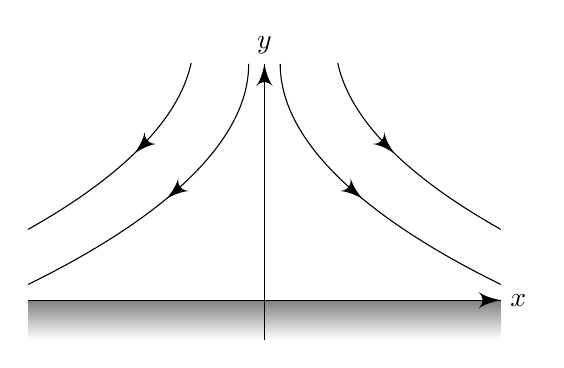
\begin{tikzpicture}
      \fill [gray, path fading=south] (-3, 0) rectangle (3, -0.5);
      \draw [->] (-3, 0) -- (3, 0) node [right] {$x$};
      \draw [->] (0, -0.5) -- (0, 3) node [above] {$y$};

      \draw [->-=0.5, rotate=90](3, 0.2) parabola (0.2, 3);
      \draw [->-=0.5, xscale=-1, rotate=90](3, 0.2) parabola (0.2, 3);

      \clip (-3, 3) rectangle (3, 0);
      \draw [->-=0.5, rotate=90](3.3, 0.9) parabola (0.9, 3);
      \draw [->-=0.5, xscale=-1, rotate=90](3.3, 0.9) parabola (0.9, 3);
    \end{tikzpicture}
  \end{center}
  The boundary conditions as $y \to \infty$ gives us a picture of what is going on at large $y$, as shown in the diagram, but near the boundary, the velocity has to start to vanish. So we would want to solve the equations to see what happens near the boundary.

  Again, this problem does not have any extrinsic length scale. So we can seek a similarity solution in terms of
  \[
    \eta = \frac{y}{\delta}, \quad \delta = \sqrt{\frac{\nu}{E}}.
  \]
  First of all, we make sure this is the right similarity solution. We show that $\delta$ has dimensions of length:
  \begin{itemize}
    \item The dimension of $E$ is $[E] = T^{-1}$
    \item The dimension of $\nu$ is $[\nu] = L^2 T^{-1}$.
  \end{itemize}
  Hence
  \[
    \left[\frac{E}{\nu}\right] = L^2,
  \]
  and $\delta$ has dimension $L$. Therefore $\eta = \frac{y}{\delta}$ is dimensionless.

  Note that we make $\eta$ a function of $y$ instead of a function of $x$ so that we can impose the boundary condition as $y \to \infty$.

  What would the similarity solution look like? Applying the incompressibility conditions $\nabla \cdot \mathbf{u} = 0$, it must be of the form
  \[
    \mathbf{u} = (u, v, 0) = (Ex g'(\nu), -E \delta g(\eta), 0).
  \]
  To check this is really incompressible, we can find the streamfunction. It turns out it is given by
  \[
    \psi = \sqrt{\nu E} x g(\eta).
  \]
  We can compute
  \[
    u = \frac{\partial \psi}{\partial t} = \sqrt{\nu E} x g'(\eta) \frac{1}{\delta} = Ex g'(\eta),
  \]
  and similarly for the $y$ component. So this is really the streamfunction. Therefore we must have $\nabla \cdot \mathbf{u} = 0$. Alternatively, we can simply compute $\nabla \cdot \mathbf{u}$ and find it to be zero.

  Finally, we look at the Navier-Stokes equations. The $x$ and $y$ components are
  \begin{align*}
    u \frac{\partial u}{\partial x} + v \frac{\partial u}{\partial y} &= -\frac{1}{\rho}\frac{\partial p}{\partial x} + \nu \left(\frac{\partial^2 u}{\partial x^2} + \frac{\partial^2 u}{\partial y^2}\right)\\
    u \frac{\partial v}{\partial x} + v \frac{\partial v}{\partial y} &= -\frac{1}{\rho}\frac{\partial p}{\partial y} + \nu \left(\frac{\partial^2 v}{\partial x^2} + \frac{\partial^2 v}{\partial y^2}\right).
  \end{align*}
  Substituting our expression for $u$ and $v$, we get
  \[
    Ex g'E g' - E \delta g E x g'' \frac{1}{\delta} = -\frac{1}{\rho} \frac{\partial p}{\partial x} - \nu E xg''' \frac{1}{\delta^2}.
  \]
  Some tidying up gives
  \[
    E^2 x(g'^2 - gg'') = -\frac{1}{\rho} \frac{\partial p}{\partial x} - E^2 x g'''.
  \]
  We can do the same thing for the $y$-component, and get
  \[
    E\sqrt{\nu E}gg' = -\frac{1}{\rho} \frac{\partial p}{\partial y} - E\sqrt{\nu E}g''.
  \]
  So we've got two equations for $g$ and $p$. The trick is to take the $y$ derivative of the first, and $x$ derivative of the second, and we can use that to eliminate the $p$ terms. Then we have
  \[
    g'g'' - gg''' = g^{(4)}.
  \]
  So we have a single equation for $g$ that we shall solve.

  We now look at our boundary conditions. The no-slip condition gives $\mathbf{u} = \mathbf{0}$ on $y = 0$. So $g'(0) = g(0) = 0$ when $\eta = 0$.

  As as $y \to \infty$, the boundary conditions for $\mathbf{u}$ gives $g'(\eta) \to 1$, $g(\eta) \to \eta$ as $\eta \to \infty$.

  All dimensional variables are absorbed into the scaled variables $g$ and $\eta$. So we only have to solve the ODE once. The far field velocity $\mathbf{u} = (Ex, -E y, 0)$ is reached to a very good approximation when
  \[
    \eta \gtrsim 1,\quad y \gtrsim \delta = \frac{\eta}{E}.
  \]
  \begin{center}
    \begin{tikzpicture}
      \draw [->] (-0.5, 0) -- (5, 0) node [right] {$\eta$};
      \draw [->] (0, -0.5) -- (0, 2.5) node [above] {$g'(\eta)$};
      \draw (0, 0) .. controls (1, 0) and (1, 2) .. (3, 2) -- (5, 2);
      \draw [dashed] (0, 2) -- (3, 2);

      \draw [<->] (0, 1) -- (3, 1) node [pos=0.5, fill=white] {$\delta = O(1)$};
    \end{tikzpicture}
  \end{center}
  We get the horizontal velocity profile as follows:
  \begin{center}
    \begin{tikzpicture}
      \draw [->] (-0.5, 0) -- (4, 0) node [right] {$x$};
      \draw [->] (0, -0.5) -- (0, 3) node [above] {$y$};

      \draw (1, 0) arc(270:360:1 and 1.5) -- (2, 3) node [pos=0.5, right] {$Ex$};

      \draw [dashed] (-1, 1.5) -- (4, 1.5);

      \draw [<->] (3, 0) -- (3, 1.5) node [pos=0.5, fill=white] {$\delta$};

      \foreach \x in {0.55, 1.1} {
        \pgfmathsetmacro\y{sqrt(1 - (1 - \x/1.5)^2)};
        \draw [-latex'] (1, \x) -- +(\y, 0);
      }
    \end{tikzpicture}
  \end{center}
  At the scale $\delta$, we get a Reynolds number of
  \[
    Re_\delta = \frac{U\delta}{\nu}\sim O(1).
  \]
  This is the \emph{boundary layer}. For a larger extrinsic scale $L \gg \delta$, we get
  \[
    Re_L = \frac{UL}{2} \gg 1.
  \]
  When interested in flow on scales much larger than $\delta$, we ignore the region $y < \delta$ (since it is small), and we imagine a rigid boundary at $y = \delta$ at which the no-slip condition does not apply.

  When $Re_L \gg 1$, we solve the Euler equations, namely
  \begin{align*}
    \rho \frac{\D \mathbf{u}}{\D t} &= - \nabla p + \mathbf{f}\\
    \nabla \cdot \mathbf{u} &= 0.
  \end{align*}
  We still have a boundary condition --- we don't allow fluid to flow \emph{through} the boundary. So we require
  \[
    \mathbf{u}\cdot \mathbf{n} = 0\quad\text{at a stationary rigid boundary}.
  \]
  The no-slip condition is no longer satisfied.

  It is an exercise for the reader to show that $\mathbf{u} = (Ex, -Ey, 0)$ satisfies the Euler equations in $y > 0$ with a rigid boundary of $y = 0$, with
  \[
    p = p_0 - \frac{1}{2} \rho E^2(x^2 + y^2).
  \]
  We can plot the curves of constant pressure, as well as the streamlines:
  \begin{center}
    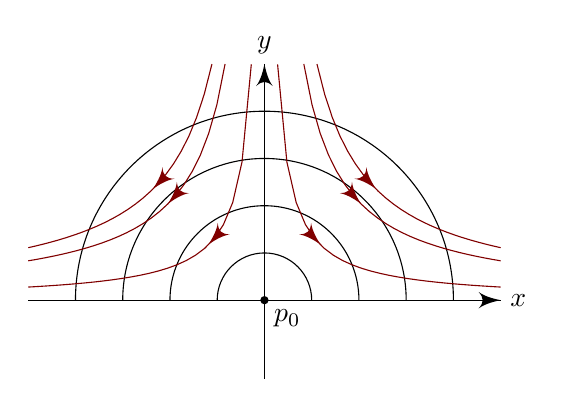
\begin{tikzpicture}
      \draw [->] (-3, 0) -- (3, 0) node [right] {$x$};
      \draw [->] (0, -1) -- (0, 3) node [above] {$y$};
      \foreach \r in {0.6, 1.2, 1.8, 2.4} {
        \draw (\r, 0) arc(0:180:\r);
      }
      \node [circ] {};
      \node [anchor = north west] {$p_0$};

      \draw [mred, ->-=0.5, domain=0.167:3] plot (\x, {0.5/\x});
      \draw [mred, ->-=0.5, domain=0.5:3] plot (\x, {1.5/\x});
      \draw [mred, ->-=0.5, domain=0.667:3] plot (\x, {2/\x});

      \draw [mred, ->-=0.5, domain=0.167:3] plot ({-\x}, {0.5/\x});
      \draw [mred, ->-=0.5, domain=0.5:3] plot ({-\x}, {1.5/\x});
      \draw [mred, ->-=0.5, domain=0.667:3] plot ({-\x}, {2/\x});
    \end{tikzpicture}
  \end{center}
  As a flow enters from the top, the pressure keeps increases, and this slows down the flow. We say the $y$-pressure gradient is \emph{adverse}. As it moves down and flows sideways, the pressure \emph{pushes} the flow. So the $x$-pressure gradient is \emph{favorable}.

  At the origin, the velocity is zero, and this is a \emph{stagnation point}. This is also the point of highest pressure. In general, velocity is high at low pressures and low at high pressures.
\end{eg}

\subsection{Momentum equation for inviscid (\texorpdfstring{$\nu = 0$}{nu = 0}) incompressible fluid}
We are now going to derive the Navier-Stokes equation in the special case where viscosity is assumed to vanish. We will derive this by considering the change in momentum.

Consider an arbitrary volume $\mathcal{D}$ with boundary $\partial \mathcal{D}$ and outward pointing normal $\mathbf{n}$.
\begin{center}
  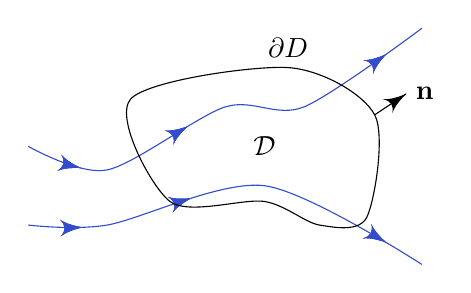
\begin{tikzpicture}
    \draw [mblue, ->-=0.13, ->-=0.4, ->-=0.9] plot [smooth] coordinates {(-3, 0) (-2, -0.3) (-0.5, 0.5) (0.5, 0.5) (2, 1.5)};
    \draw [mblue, ->-=0.13, ->-=0.4, ->-=0.9] plot [smooth] coordinates {(-3, -1) (-2, -1) (0, -0.5) (2, -1.5)};
    \draw plot [smooth cycle] coordinates {(-1.2, -0.7) (0, -0.7) (0.7, -1) (1.3, -0.9) (1.4, 0.4) (0.3, 1) (-1.7, 0.6)};
    \node at (0, 0) {$\mathcal{D}$};
    \node [above] at (0.3, 1) {$\partial D$};
    \draw [->] (1.4, 0.4) -- +(0.4, 0.2666) node [right] {$\mathbf{n}$};
  \end{tikzpicture}
\end{center}
The total momentum of the fluid in $\mathcal{D}$ can change owing to four things:
\begin{enumerate}
  \item Momentum flux across the boundary $\partial \mathcal{D}$;
  \item Surface pressure forces;
  \item Body forces;
  \item Viscous surface forces.
\end{enumerate}
We will ignore the last one. We can then write the rate of change of the total momentum as
\[
  \frac{\d}{\d t} \int_{\mathcal{D}} \rho \mathbf{u} \;\d V = -\int_{\partial \mathcal{D}} \rho \mathbf{u} (\mathbf{u}\cdot \mathbf{n}) \;\d S - \int_{\partial \mathcal{D}} p \mathbf{n}\;\d S + \int_{\mathcal{D}} \mathbf{f}\;\d V.
\]
It is helpful to write this in suffix notation. In this case, the equation becomes
\[
  \frac{\d}{\d t} \int_{\mathcal{D}} \rho u_i \;\d V = -\int_{\partial \mathcal{D}} \rho u_i u_j n_j \;\d S - \int_{\partial \mathcal{D}} - p n_i \;\d S + \int_{\mathcal{D}} f_i \;\d V.
\]
Just as in the case of mass conservation, we can use the divergence theorem to write
\[
  \int_{\mathcal{D}} \left(\rho \frac{\partial u_i}{\partial t} + \rho \frac{\partial}{\partial x_j} (u_i u_j)\right)\;\d V = \int_{\mathcal{D}} \left(-\frac{\partial p}{\partial x_i} + f_i\right) \;\d V.
\]
Since $\mathcal{D}$ is arbitrary, we must have
\[
  \rho \frac{\partial u_i}{\partial t} + \rho \frac{\partial u_i}{\partial x_j} + \rho u_i \frac{\partial u_j}{\partial x_j} = -\frac{\partial p}{\partial x_i} + f_i.
\]
The last term on the left is the divergence of $\mathbf{u}$, which vanishes by incompressibility, and the remaining terms is just the material derivative of $\mathbf{u}$. So we get
\begin{prop}[Euler momentum equation]
  \[
    \rho \frac{\D \mathbf{u}}{\D t} = - \nabla p + \mathbf{f}.
  \]
\end{prop}
This is just the equation we get from the Navier-Stokes equation by ignoring the viscous terms. However, we were able to derive this directly from momentum conservation.

We can further derive some equations from this.

For conservative forces, we can write $\mathbf{f} = -\nabla \chi$, where $\chi$ is a scalar potential. For example, gravity can be given by $\mathbf{f} = \rho \mathbf{g} = \nabla (\rho \mathbf{g}\cdot \mathbf{x})$ (for $\rho$ constant). So $\chi = - \rho \mathbf{g}\cdot \mathbf{x} = g \rho z$ if $\mathbf{g} = (0, 0, -g)$.

In the case of a steady flow, $\frac{\partial \mathbf{u}}{\partial t}$ vanishes. Then the momentum equation becomes
\[
  0 = -\int_{\partial \mathcal{D}} \rho \mathbf{u} (\mathbf{u} \cdot \mathbf{n}) \;\d S - \int_{\partial \mathcal{D}}p \mathbf{n} \;\d S - \int_{\mathcal{D}} \nabla \chi \;\d V.
\]
We can then convert this to
\begin{prop}[Momentum integral for steady flow]
  \[
    \int_{\partial \mathcal{D}} (\rho \mathbf{u} (\mathbf{u}\cdot \mathbf{n}) + p \mathbf{n} + \chi \mathbf{n}) \;\d S = 0.
  \]
\end{prop}
Alternatively, we notice the vector identity
\[
  \mathbf{u}\times (\nabla \times \mathbf{u}) = \nabla\left(\frac{1}{2}|\mathbf{u}|^2\right) - \mathbf{u}\cdot \nabla \mathbf{u}.
\]
We use this to rewrite the Euler momentum equation as
\[
  \rho \frac{\partial \mathbf{u}}{\partial t} + \rho \nabla \left(\frac{1}{2}|\mathbf{u}|^2\right) - \rho \mathbf{u}\times (\nabla \times \mathbf{u}) = -\nabla p - \nabla \chi.
\]
Dotting with $\mathbf{u}$, the last term on the left vanishes, and we get
\begin{prop}[Bernoulli's equation]
  \[
    \frac{1}{2}\rho \frac{\partial|\mathbf{u}|^2}{\partial t} = -\mathbf{u}\cdot \nabla \left(\frac{1}{2} \rho |\mathbf{u}|^2 + p + \chi\right).
  \]
\end{prop}
Note also that this tells us that high velocity goes with low pressure; low pressure goes with high velocity.

In the case where we have a steady flow, we know
\[
  H = \frac{1}{2}\rho |\mathbf{u}|^2 + p + \chi
\]
is constant along streamlines.

Even if the flow is not steady, we can still define the value $H$, and then we can integrate Bernoulli's equation over a volume $\mathcal{D}$ to obtain
\[
  \frac{\d}{\d t}\int_{\mathcal{D}} \frac{1}{2}\rho |\mathbf{u}|^2 \;\d V = -\int_{\partial \mathcal{D}} H \mathbf{u}\cdot \mathbf{n} \;\d S.
\]
So $H$ is the transportable energy of the flow.

\begin{eg}
  Consider a pipe with a constriction. Ignore the vertical pipes for the moment --- they are there just so that we can measure the pressure in the fluid, as we will later see.
  \begin{center}
    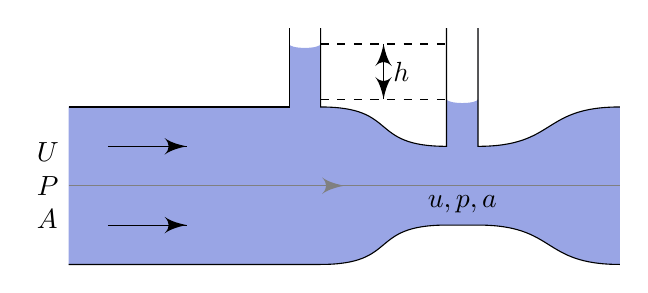
\begin{tikzpicture}
      \fill [mblue, opacity=0.5] (-3, 2) -- (-0.2, 2) -- (-0.2, 2.8) arc(180:360:0.2 and 0.05) -- (0.2, 3) -- (0.2, 2) .. controls (1.2, 2) and (0.8, 1.5) .. (1.8, 1.5) -- (1.8, 2.1) arc(180:360:0.2 and 0.05) -- (2.2, 3) -- (2.2, 1.5) .. controls (3.2, 1.5) and (3, 2) .. (4, 2) -- (4, 0) .. controls (3, 0) and (3.2, 0.5) .. (2.2, 0.5) -- (1.8, 0.5) .. controls (0.8, 0.5) and (1.2, 0) .. (0.2, 0) -- (-3, 0) -- cycle;

      \draw [dashed] (0.2, 2.1) -- (1.8, 2.1);
      \draw [dashed] (0.2, 2.8) -- (1.8, 2.8);

      \draw [<->] (1, 2.1) -- (1, 2.8) node [pos=0.5, right] {$h$};

      \draw (-3, 2) -- (-0.2, 2) -- (-0.2, 3);
      \draw (0.2, 3) -- (0.2, 2) .. controls (1.2, 2) and (0.8, 1.5) .. (1.8, 1.5) -- (1.8, 3);
      \draw (-3, 0) -- (0.2, 0) .. controls (1.2, 0) and (0.8, 0.5) .. (1.8, 0.5) -- (2.2, 0.5) .. controls (3.2, 0.5) and (3, 0) .. (4, 0);
      \draw (2.2, 3) -- (2.2, 1.5) .. controls (3.2, 1.5) and (3, 2) .. (4, 2);

      \draw [gray, ->-=0.5] (-3, 1) -- (4, 1);

      \node [align=left, left] at (-3, 1) {$U$\\$P$\\$A$};
      \node [below] at (2, 1) {$u, p, a$};

      \draw [->] (-2.5, 1.5) -- +(1, 0);
      \draw [->] (-2.5, 0.5) -- +(1, 0);
    \end{tikzpicture}
  \end{center}
  Suppose at the left, we have a uniform speed $U$, area $A$ and pressure $P$. In the middle constricted area, we have speed $u$, area $a$ and pressure $p$.

  By the conservation of mass, we have
  \[
    q = UA = ua.
  \]
  We apply Bernoulli along the central streamline, using the fact that $H$ is constant along streamlines. We can omit the body force $\chi = \rho gy$, since this is the same at both locations. Then we get
  \[
    \frac{1}{2}\rho U^2 + P = \frac{1}{2} \rho u^2 + p.
  \]
  Replacing our $U$ with $q/A$ and $u$ with $q/a$, we obtain
  \[
    \frac{1}{2} \rho \left(\frac{q}{A}\right)^2 + P = \frac{1}{2} \rho \left(\frac{q}{a}\right)^2 + p.
  \]
  Rearranging gives
  \[
    \left(\frac{1}{A^2} - \frac{1}{a^2}\right)q^2 = \frac{2(p - P)}{\rho}.
  \]
  We see there is a difference in pressure due to the difference in area. This is balanced by the difference in heights $h$. Using the $y$-momentum equation, we get
  \[
    \left(\frac{1}{A^2} - \frac{1}{a^2}\right)q^2 = \frac{2(p - P)}{\rho} = -2gh.
  \]
  Then we obtain
  \[
    q = \sqrt{2gh} \frac{Aa}{\sqrt{A^2 - a^2}}.
  \]
  Therefore we can measure $h$ in order to find out the flow rate. This allows us to measure fluid velocity just by creating a constriction and then putting in some pipes.
\end{eg}

\begin{eg}[Force on a fire hose nozzle]
  Suppose we have a fire hose nozzle like this:
  \begin{center}
    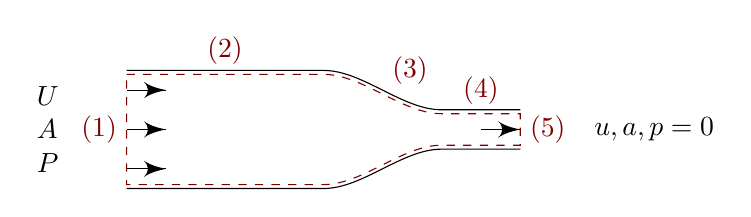
\begin{tikzpicture}
      \draw (-3, 0.75) -- (-0.5, 0.75) .. controls (0, 0.75) and (0.5, 0.25) .. (1, 0.25) -- (2, 0.25);
      \draw (-3, -0.75) -- (-0.5, -0.75) .. controls (0, -0.75) and (0.5, -0.25) .. (1, -0.25) -- (2, -0.25);

      \draw [->] (-3, 0.5) -- +(0.5, 0);
      \draw [->] (-3, 0) -- +(0.5, 0);
      \draw [->] (-3, -0.5) -- +(0.5, 0);

      \draw [->] (1.5, 0) -- +(0.5, 0);

      \draw [mred, dashed] (-3, 0.7) -- (-0.5, 0.7) node [pos=0.5, above] {$(2)$}.. controls (0, 0.7) and (0.5, 0.2) .. (1, 0.2) node [pos=0.5, anchor = south west] {$(3)$} -- (2, 0.2) node [pos=0.5, above] {$(4)$} -- (2, -0.2) node [pos=0.5, right] {$(5)$} -- (1, -0.2) .. controls (0.5, -0.2) and (0, -0.7) .. (-0.5, -0.7) -- (-3, -0.7) -- cycle node [pos=0.5, left] {$(1)$};

      \node [align=left] at (-4, 0) {$U$\\$A$\\$P$};
      \node at (3.7, 0) {$u, a, p = 0$};
    \end{tikzpicture}
  \end{center}
  We consider the steady-flow equation and integrate along the surface indicated above. We integrate each section separately. The end $(1)$ contributes
  \[
    \rho U(-U)A - PA.
  \]
  On $(2)$, everything vanishes. On $(3)$, the first term vanishes since the velocity is parallel to the surface. Then we get a contribution of
  \[
    0 + \int_{\mathrm{nozzle}} p \mathbf{n}\cdot \hat{\mathbf{x}}\;\d S.\tag{3}
  \]
  Similarly, everything in $(4)$ vanishes. Finally, on $(5)$, noting that $p = 0$, we get
  \[
    \rho u^2 a.
  \]
  By the steady flow equation, we know these all sum to zero. Hence, the force on the nozzle is just
  \[
    F = \int_{\mathrm{nozzle}} p\mathbf{n}\cdot \hat{\mathbf{x}}\;\d S = \rho AU^2 - \rho au^2 + PA.
  \]
  We can again apply Bernoulli along a streamline in the middle, which says
  \[
    \frac{1}{2}\rho U^2 + P = \frac{1}{2} \rho u^2.
  \]
  So we can get
  \[
    F = \rho AU^2 - \rho au^2 + \frac{1}{2} \rho A(u^2 - U^2) = \frac{1}{2} \rho\frac{A}{a^2}q^2 \left(1 - \frac{a}{A}\right)^2.
  \]
  Let's now put some numbers in. Suppose $A = (0.1)^2 \pi\SI{}{\meter\squared}$ and $a = (0.05)^2 \pi\SI{}{\meter\squared}$. So we get
  \[
    \frac{A}{a} = 4.
  \]
  A typical fire hose has a flow rate of
  \[
    q = \SI{0.01}{\meter\cubed\per\second}.
  \]
  So we get
  \[
    F = \frac{1}{2} \cdot 1000 \cdot \frac{4}{\pi/40} \cdot 10^{-4} \cdot \left(\frac{3}{4}\right)^2 \approx \SI{14}{N}.
  \]
\end{eg}

\subsection{Linear flows}
Suppose we have a favorite point $\mathbf{x}_0$. Near the point $\mathbf{x}_0$, it turns out we can break up the flow into three parts --- uniform flow, pure strain, and pure rotation.

To do this, we take the Taylor expansion of $\mathbf{u}$ about $\mathbf{x}_0$:
\begin{align*}
  \mathbf{u}(\mathbf{x}) &= \mathbf{u}(\mathbf{x}_0) + (\mathbf{x} - \mathbf{x}_0) \cdot \nabla \mathbf{u}(\mathbf{x}_0) + \cdots\\
  &= \mathbf{u}_0 + \mathbf{r}\cdot \nabla \mathbf{u}_0,
\end{align*}
with $\mathbf{r} = \mathbf{x} - \mathbf{x}_0$ and $\mathbf{u}_0 = \mathbf{u}(\mathbf{x}_0)$. This is a linear approximation to the flow field.

We can do something more about the $\nabla \mathbf{u}$ term. This is a rank-2 tensor, i.e.\ a matrix, and we can split it into its symmetric and antisymmetric parts:
\[
  \nabla \mathbf{u} = \frac{\partial u_i}{\partial x_j} = E_{ij} + \Omega_{ij} = E + \Omega,
\]
where
\begin{align*}
  E_{ij} &= \frac{1}{2}\left(\frac{\partial u_i}{\partial x_j} + \frac{\partial u_j}{\partial x_i}\right),\\
  \Omega_{ij} &=\frac{1}{2}\left(\frac{\partial u_i}{\partial x_j} - \frac{\partial u_j}{\partial x_i}\right),
\end{align*}
We can write the second part in terms of the vorticity. Recall we have defined the vorticity as
\[
  \boldsymbol\omega = \nabla \times \mathbf{u}.
\]
Then we have
\[
  \boldsymbol\omega \times \mathbf{r} = (\nabla \times \mathbf{u}) \times \mathbf{r} = r_j \left(\frac{\partial u_i}{\partial x_j} - \frac{\partial u_j}{\partial x_i}\right) = 2 \Omega_{ij}r_j.
\]
So we can write
\[
  \mathbf{u} = \mathbf{u}_0 + E \mathbf{r} + \frac{1}{2} \boldsymbol\omega \times \mathbf{r}.
\]
The first component is uniform flow; the second is the strain field; and the last is the rotation component.
\begin{center}
  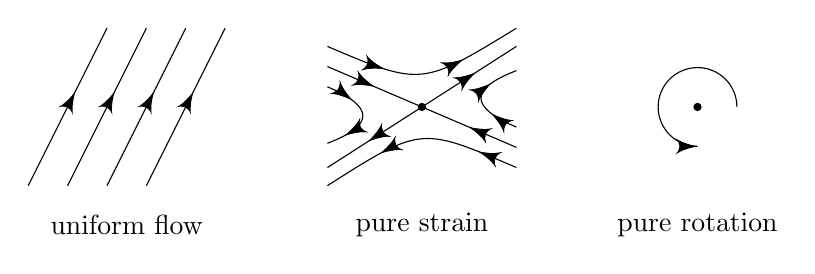
\begin{tikzpicture}
    \foreach \x in {0,0.5,1,1.5} {
      \draw [->-=0.6] (\x, 0) -- +(1, 2);
    }
    \node at (1.25, -0.5) {uniform flow};

    \begin{scope}[shift={(5, 1)}, xscale=0.3, yscale=0.7692]
      \draw [->-=0.785, -<-=0.215] (-4, -1) -- (4, 1);
      \draw [->-=0.25, -<-=0.75] (-4, 0.667) -- (4, -0.667);

      \draw [->- = 0.3, ->- = 0.7] (-4, 1) .. controls (0, 0.333) and (0, 0.35) .. (4, 1.3);
      \draw [-<- = 0.3, -<- = 0.8] (-4, -1.3) .. controls (0, -0.3) and (0, -0.333) .. (4, -1);

      \draw [->- = 0.3, ->- = 0.8] (-4, 0.333) .. controls (-2, 0) and (-2, -0.3) .. (-4, -0.6);
      \draw [->- = 0.3, ->- = 0.7] (4, -0.333) .. controls (2, 0) and (2, 0.3) .. (4, 0.6);
      \node [circ] at (0, 0) {};
    \end{scope}
    \node at (5, -0.5) {pure strain};

    \node [circ] at (8.5, 1) {};

    \draw [->] (9, 1) arc(0:270:0.5);

    \node at (8.5, -0.5) {pure rotation};
  \end{tikzpicture}
\end{center}
Since we have an incompressible fluid, we have $\nabla \cdot \mathbf{u} = 0$. So $E$ has zero trace, i.e.\ if
\[
  E =
  \begin{pmatrix}
    E_1 & 0 & 0\\
    0 & E_2 & 0\\
    0 & 0 & E_3
  \end{pmatrix},
\]
then $E_1 + E_2 + E_3 = 0$. This justifies the picture above.

\subsection{Vorticity equation}
The Navier-Stokes equation tells us how the velocity changes with time. Can we obtain a similar equation for the vorticity? Consider the Navier-Stokes equation for a viscous fluid,
\[
  \rho\left(\frac{\partial \mathbf{u}}{\partial t} + \mathbf{u}\cdot \nabla \mathbf{u}\right) = -\nabla p - \nabla \chi + \mu \nabla^2 \mathbf{u}
\]
We use a vector identity
\[
  \mathbf{u}\cdot \nabla \mathbf{u} = \frac{1}{2}\nabla |\mathbf{u}^2| - \mathbf{u}\times \boldsymbol\omega,
\]
and take the curl of the above equation to obtain
\[
  \frac{\partial \boldsymbol\omega}{\partial t} - \nabla \times (\mathbf{u}\times \boldsymbol\omega) = \nu \nabla^2 \boldsymbol\omega,
\]
exploiting the fact that the curl of a gradient vanishes. We now use the fact that
\[
  \nabla \times (\mathbf{u}\times \boldsymbol\omega) = (\nabla \cdot \boldsymbol\omega) \mathbf{u} + \boldsymbol\omega \cdot \nabla \mathbf{u} - (\nabla \cdot \mathbf{u}) \boldsymbol\omega - \mathbf{u}\cdot \nabla \boldsymbol\omega.
\]
The divergence of a curl vanishes, and so does $\nabla \cdot \mathbf{u}$ by incompressibility. So we get
\[
  \frac{\partial \boldsymbol\omega}{\partial t} + \mathbf{u}\cdot \nabla \boldsymbol\omega - \boldsymbol\omega \cdot \nabla \mathbf{u} = \nu \nabla^2 \boldsymbol \omega.
\]
Now we use the definition of the material derivative, and rearrange terms to obtain
\begin{prop}[Vorticity equation]
  \[
    \frac{\D \boldsymbol\omega}{\D t} = \boldsymbol\omega \cdot \nabla \mathbf{u} + \nu \nabla^2 \boldsymbol\omega.
  \]
\end{prop}
Hence, the rate of change of vorticity of a fluid particle is caused by $\boldsymbol\omega \cdot \nabla \mathbf{u}$ (amplification by stretching or twisting) and $\nu \nabla^2 \boldsymbol\omega$ (dissipation of vorticity by viscosity). The second term also allows for generation of vorticity at boundaries by the no-slip condition. This will be explained shortly.

Consider an inviscid fluid, where $\nu = 0$. So we are left with
\[
  \frac{\D \boldsymbol\omega}{\D t} = \boldsymbol\omega \cdot \nabla \mathbf{u}.
\]
So if we take the dot product with $\boldsymbol\omega$, we get
\begin{align*}
  \frac{\D}{\D t}\left(\frac{1}{2} |\boldsymbol\omega|^2\right) &= \boldsymbol\omega \cdot \nabla u \cdot \boldsymbol\omega\\
  &= \boldsymbol\omega (E + \Omega) \boldsymbol\omega\\
  &= \omega_i (E_{ij} + \Omega_{ij}) \omega_j.
\end{align*}
Since $\omega_i \omega_j$ is symmetric, while $\Omega_{ij}$ is antisymmetric, the second term vanishes. In the principal axes, $E$ is diagonalizable. So we get
\[
  \frac{\D}{\D t} \left(\frac{1}{2} |\boldsymbol\omega|^2\right) = E_1 \omega_1^2 + E_2 \omega_2^2 + E_3 \omega_3^2.
\]
wlog, we assume $E_1 > 0$ (since the $E_i$'s sum to $0$), and imagine $E_2, E_3 < 0$. So the flow is stretched in the $\mathbf{e}_1$ direction and compressed radially. We consider what happens to a vortex in the direction of the stretching, $\boldsymbol\omega = (\omega_1, 0, 0)$. We then get
\[
  \frac{\D}{\D t}\left(\frac{1}{2}\omega_1^2\right) = E_1 \omega_1^2.
\]
So the vorticity grows exponentially. This is vorticity amplification by stretching. This is not really unexpected --- as the fluid particles have to get closer to the axis of rotation, they have to rotate faster, by the conservation of angular momentum.

This is in general true --- vorticity increases as the length of a material line increases. To show this, we consider two neighbouring (Lagrangian) fluid particles, $\mathbf{x}_1(t), \mathbf{x}_2(t)$. We let $\delta\boldsymbol\ell(t) = \mathbf{x}_2(t) - \mathbf{x}_1(t)$. Note that
\[
  \frac{\D \mathbf{x}_2(t)}{\D t} = \mathbf{u}_2(\mathbf{x}_2),\quad \frac{\D \mathbf{x}_1(t)}{\D t} = \mathbf{u}_1(\mathbf{x}_1).
\]
Therefore
\[
  \frac{\D \delta \boldsymbol\ell(t)}{\D t} = \mathbf{u}(\mathbf{x}_2) - \mathbf{u}(\mathbf{x}_1) = \delta \boldsymbol\ell \cdot \nabla \mathbf{u},
\]
by taking a first-order Taylor expansion. This is exactly the same equation as that for $\boldsymbol\omega$ in an inviscid fluid. So vorticity increases as the length of a material line increases.

Note that the vorticity is generated by viscous forces near boundaries.
\begin{center}
  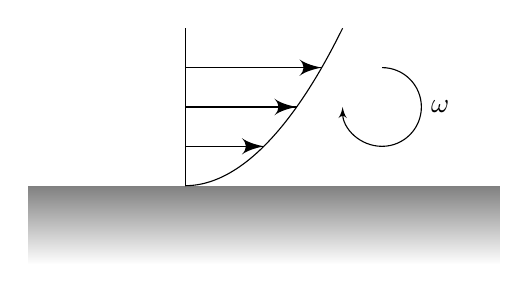
\begin{tikzpicture}
    \fill [gray, path fading=south] (0, 0) rectangle (6, -1);

    \draw (2, 0) -- (2, 2);
    \draw (2, 0) parabola (4, 2);

    \foreach \x in {0.5,1,1.5} {
      \pgfmathsetmacro\y{sqrt(2 * \x)};
      \draw [->] (2, \x) -- +(\y, 0);
    }
    \draw [-latex'] (4.5, 1.5) arc(90:-180:0.5);
    \node at (5, 1) [right] {$\omega$};
  \end{tikzpicture}
\end{center}
When we make the inviscid approximation, then we are losing this source of vorticity, and we sometimes have to be careful.

We have so far assumed the density is constant. If the fluid has a non-uniform density $\rho(\mathbf{x})$, then it turns out
\[
  \frac{\D \boldsymbol\omega}{\D t} = \boldsymbol\omega \cdot \nabla \mathbf{u} + \frac{1}{\rho^2} \nabla \rho \times \nabla p.
\]
This is what happens in convection flow. The difference in density drives a motion of the fluid. For example, if we have a horizontal density gradient and a vertical pressure gradient (e.g.\ we have a heater at the end of a room with air pressure varying according to height), then we get the following vorticity:
\begin{center}
  \begin{tikzpicture}
    \draw [->] (0, 3) -- (0, 0) node [below] {$\nabla p$};
    \draw [->] (-0.5, 2.5) -- +(3, 0) node [above] {$\nabla \rho$};

    \node at (-3, 1.5) {hot, light};
    \node at (3, 1.5) {cold, dense};

    \draw [-latex'] (1, 2) arc(90:-180:0.5);
    \node at (1.5, 1.5) [right] {$\omega$}; % improve
    \node at (1, 1.5) {$\times$};
  \end{tikzpicture}
\end{center}

\section{Inviscid irrotational flow}
From now on, we are going to make a further simplifying assumption. We are going to assume that our flow is is incompressible, inviscid, \emph{and} irrotational.

We first check this is a sensible assumption, in that if we start of with an irrotational flow, then the flow will continue being irrotational. Suppose we have $\nabla \times \mathbf{u} = \mathbf{0}$ at $t = 0$, and the fluid is inviscid and homogeneous (i.e.\ $\rho$ is constant). Then by the vorticity equation
\[
  \frac{\D \boldsymbol\omega}{\D t} = \boldsymbol\omega \cdot \nabla \mathbf{u} = 0.
\]
So the vorticity will keep on being zero.

In this case, we can write $\mathbf{u} = \nabla \phi$ for some $\phi$.
\begin{defi}[Velocity potential]
  The \emph{velocity potential} of a velocity $\mathbf{u}$ is a scalar function $\phi$ such that $\mathbf{u} = \nabla \phi$.
\end{defi}
Note that since we are lazy, we don't not have a negative sign in front of $\nabla \phi$, unlike, say, gravity.

If we are incompressible, then $\nabla \cdot \mathbf{u} = 0$ implies
\[
  \nabla^2 \phi = 0.
\]
So the potential satisfies Laplace's equation.

\begin{defi}[Potential flow]
  A \emph{potential flow} is a flow whose velocity potential satisfies Laplace's equation.
\end{defi}

A key property of Laplace's equation is that it is linear. So we can add two solutions up to get a third solution.

\subsection{Three-dimensional potential flows}
We will not consider Laplace's equation in full generality. Instead, we will consider some solutions with symmetry. We will thus use spherical coordinates $(r, \theta, \varphi)$. Then
\[
  \nabla^2 \phi = \frac{1}{r^2} \pd{r} \left(r^2 \frac{\partial \phi}{\partial r}\right) + \frac{1}{r^2 \sin \theta} \pd{\theta} \left(\sin \theta\frac{\partial \phi}{\partial \theta}\right) + \frac{1}{r^2 \sin^2 \theta} \frac{\partial^2 \phi}{\partial \varphi^2}.
\]
It is also useful to know what the gradient is. This is given by
\[
  \mathbf{u} = \nabla \phi = \left(\frac{\partial \phi}{\partial r}, \frac{1}{r} \frac{\partial \phi}{\partial \theta}, \frac{1}{r \sin \theta} \frac{\partial \phi}{\partial \varphi}\right).
\]
We start off with the simplest case. The simplest thing we can possibly imagine is if $\phi = \phi(r)$ depends only on $r$. So the velocity is purely radial. Then Laplace's equation implies
\[
  \frac{\partial}{\partial r}\left(r^2 \frac{\partial \phi}{\partial r}\right) = 0.
\]
So we know
\[
  \frac{\partial \phi}{\partial r} = \frac{A}{r^2}
\]
for some constant $A$. So
\[
  \phi = -\frac{A}{r} + B,
\]
where $B$ is yet another constant. Since we only care about the gradient $\nabla \phi$, we can wlog $B = 0$. So the only possible velocity potential is
\[
  \phi = -\frac{A}{r}.
\]
Then the speed, given by $\frac{\partial \phi}{\partial r}$, falls off as $\frac{1}{r^2}$.

What is the physical significance of the factor $A$? Consider the volume flux $q$ across the surface of the sphere $r = a$. Then
\[
  q = \int_S \mathbf{u}\cdot \mathbf{n} \;\d S = \int_S u_r \;\d S = \int_S \frac{\partial \phi}{\partial r} \;\d S = \int_S \frac{A}{a^2}\;\d S = 4\pi A.
\]
So we can write
\[
  \phi = -\frac{q}{4\pi r}.
\]
When $q > 0$, this corresponds to a point source of fluid. When $q < 0$, this is a point sink of fluid.

We can also derive this solution directly, using incompressibility. Since flow is incompressible, the flux through any sphere containing $0$ should be constant. Since the surface area increases as $4\pi r^2$, the velocity must drop as $\frac{1}{r^2}$, in agreement with what we obtained above.

Notice that we have
\[
  \nabla^2 \phi = q \delta(x).
\]
So $\phi$ is actually Green's function for the Laplacian.

That was not too interesting. We can consider a less general solution, where $\phi$ depends on $r$ and $\theta$ but not $\varphi$. Then Laplace's equation becomes
\[
  \nabla^2 \phi = \frac{1}{r^2} \pd{r} \left(r^2 \frac{\partial \phi}{\partial r}\right) + \frac{1}{r^2 \sin \theta} \pd{\theta} \left(\sin \theta\frac{\partial \phi}{\partial \theta}\right) = 0.
\]
As we know from IB Methods, We can use Legendre polynomials to write the solution as
\[
  \phi = \sum_{n = 0}^\infty (A_n r^n + B_n r^{-n - 1})P_n(\cos \theta).
\]
We then have
\[
  \mathbf{u} =
  \left(\frac{\partial \phi}{\partial r}, \frac{1}{r}\frac{\partial \phi}{\partial \theta},0\right).
\]
\begin{eg}
  We can look at uniform flow past a sphere of radius $a$.
  \begin{center}
    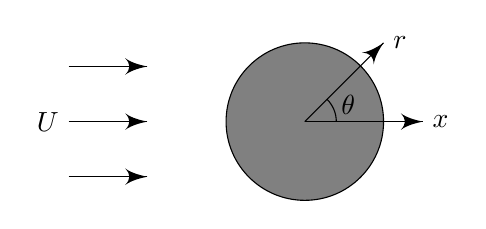
\begin{tikzpicture}
      \draw [fill=gray] circle [radius=1];
      \draw [->] (-3, 0.7) -- +(1, 0);
      \draw [->] (-3, 0) node [left] {$U$} -- +(1, 0);
      \draw [->] (-3, -0.7) -- +(1, 0);

      \draw [->] (0, 0) -- (1.5, 0) node [right] {$x$};
      \draw [->] (0, 0) -- (1, 1) node [right] {$r$};
      \draw (0.4, 0) arc(0:45:0.4) node [pos=0.7, right] {$\theta$};
    \end{tikzpicture}
  \end{center}
  We suppose the upstream flow is $\mathbf{u} = U \hat{\mathbf{x}}$. So
  \[
    \phi = Ux = Ur\cos \theta.
  \]
  So we need to solve
  \begin{align*}
    \nabla^2 \phi &= 0 & r &>a\\
    \phi&\to Ur \cos \theta & r &\to \infty\\
    \frac{\partial \phi}{\partial r}&= 0 & r&=a.
  \end{align*}
  The last condition is there to ensure no fluid flows into the sphere, i.e.\ $\mathbf{u}\cdot \mathbf{n} = 0$, for $\mathbf{n}$ the outward normal.

  Since $P_1(\cos \theta) = \cos \theta$, and the $P_n$ are orthogonal, our boundary conditions at infinity require $\phi$ to be of the form
  \[
    \phi = \left(Ar + \frac{B}{r^2}\right) \cos \theta.
  \]
  We now just apply the two boundary conditions. The condition that $\phi \to Ur \cos \theta$ tells us $A = u$, and the other condition tells us
  \[
    A - \frac{2B}{a^3} = 0.
  \]
  So we get
  \[
    \phi = U\left(r + \frac{a^3}{2r^2}\right) \cos \theta.
  \]
  We can interpret $Ur \cos \theta$ as the uniform flow, and $U \frac{a^3}{2r^2} \cos \theta$ as the dipole response due to the sphere.

  What is the velocity and pressure? We can compute the velocity to be
  \begin{align*}
    u_r &= \frac{\partial \phi}{\partial r} = U\left(1 - \frac{a^3}{r^3}\right) \cos \theta\\
    u_\theta &= \frac{1}{r} \frac{\partial \phi}{\partial \theta} = -U\left(1 + \frac{a^3}{2r^3}\right)\sin \theta.
  \end{align*}
  We notice that $u_r = u_\theta = 0$ when $\phi = 0, \pi$ and $r = a$.

  At the north and south poles, when $\theta = \pm \frac{\pi}{2}$, we get
  \[
    u_r = 0,\quad u_\theta = \pm \frac{3U}{2}.
  \]
  So the velocity is faster at the top than at the infinity boundary. This is why it is windier at the top of a hill than below.
  \begin{center}
    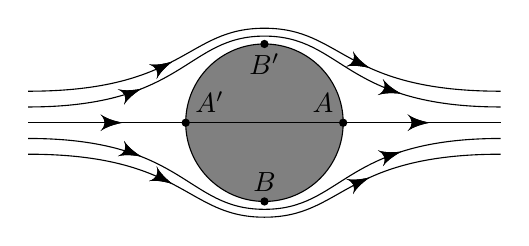
\begin{tikzpicture}
      \draw [fill=gray] circle [radius=1];
      \draw [->-=0.2, ->-=0.85] (-3, 0) -- (3, 0);
      \node [circ] at (-1, 0) {};
      \node [circ] at (1, 0) {};
      \node [anchor = south west] at (-1, 0) {$A'$};
      \node [anchor = south east] at (1, 0) {$A$};
      \node [circ] at (0, -1) {};
      \node [circ] at (0, 1) {};
      \node [above] at (0, -1) {$B$};
      \node [below] at (0, 1) {$B'$};

      \draw [->-=0.23, ->-=0.8] (-3, 0.2) .. controls (-1, 0.2) and (-1, 1.1) .. (0, 1.1) .. controls (1, 1.1) and (1, 0.2) .. (3, 0.2);
      \draw [->-=0.3, ->-=0.73] (-3, 0.4) .. controls (-1, 0.4) and (-1, 1.2) .. (0, 1.2) .. controls (1, 1.2) and (1, 0.4) .. (3, 0.4);
      \draw [->-=0.23, ->-=0.8] (-3, -0.2) .. controls (-1, -0.2) and (-1, -1.1) .. (0, -1.1) .. controls (1, -1.1) and (1, -0.2) .. (3, -0.2);
      \draw [->-=0.3, ->-=0.73] (-3, -0.4) .. controls (-1, -0.4) and (-1, -1.2) .. (0, -1.2) .. controls (1, -1.2) and (1, -0.4) .. (3, -0.4);
    \end{tikzpicture}
  \end{center}
  Note that the streamlines are closer to each other near the top since the velocity is faster.

  To obtain the pressure on the surface of the sphere, we apply Bernoulli's equation on a streamline to the surface $(a, \theta)$.

  Comparing with what happens at infinity, we get
  \[
    p_\infty + \frac{1}{2} \rho U^2 = p + \frac{1}{2}\rho U^2 \frac{9}{4} \sin^2 \theta.
  \]
  Thus, the pressure at the surface is
  \[
    p = p_\infty + \frac{1}{2}\rho U^2 \left(1 - \frac{9}{4} \sin^2 \theta\right).
  \]
  At $A$ and $A'$, we have
  \[
    p = p_\infty + \frac{1}{2}\rho U^2.
  \]
  At $B$ and $B'$, we find
  \[
    p = p_\infty - \frac{5}{8} \rho U^2.
  \]
  Note that the pressure is a function of $\sin^2 \theta$. So the pressure at the back of the sphere is exactly the same as that at the front. Thus, if we integrate the pressure around the whole surface, we get $0$. So the fluid exerts no net force on the sphere! This is d'Alemberts' paradox. This is, of course, because we have ignored viscosity.

  In practice, for a solid sphere in a viscous fluid at high Reynolds numbers, the flow looks very similar upstream, but at some point after passing the sphere, the flow separates and forms a \emph{wake} behind the sphere. At the wake, the pressure is approximately $p_\infty$. The separation is caused by the adverse pressure gradient at the rear.
   \begin{center}
    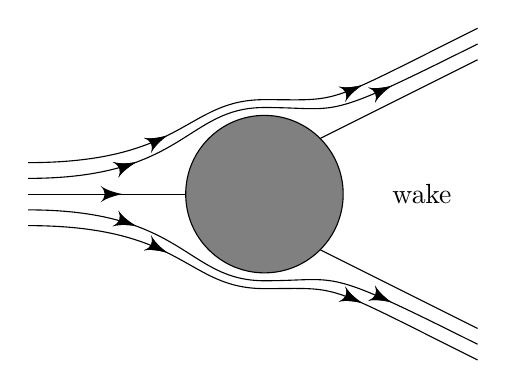
\begin{tikzpicture}
      \draw [fill=gray] circle [radius=1];
      \draw [->-=0.6] (-3, 0) -- (-1, 0);

      \draw (0.707, 0.707) -- +(2, 1);
      \draw (0.707, -0.707) -- +(2, -1);

      \draw [->-=0.23, ->-=0.8] (-3, 0.2) .. controls (-1, 0.2) and (-1, 1.1) .. (0, 1.1) .. controls (1, 1.1) and (0.707, 0.907) .. (2.707, 1.907);
      \draw [->-=0.3, ->-=0.73] (-3, 0.4) .. controls (-1, 0.4) and (-1, 1.2) .. (0, 1.2) .. controls (1, 1.2) and (0.707, 1.107) .. (2.707, 2.107);
      \draw [->-=0.23, ->-=0.8] (-3, -0.2) .. controls (-1, -0.2) and (-1, -1.1) .. (0, -1.1) .. controls (1, -1.1) and (0.707, -0.907) .. (2.707, -1.907);
      \draw [->-=0.3, ->-=0.73] (-3, -0.4) .. controls (-1, -0.4) and (-1, -1.2) .. (0, -1.2) .. controls (1, -1.2) and (0.707, -1.107) .. (2.707, -2.107);

      \node at (2, 0) {wake};
    \end{tikzpicture}
  \end{center}
  Empirically, we find the force is
  \[
    F = C_D \frac{1}{2} \rho U^2\pi \alpha^2,
  \]
  where $C_D$ is a dimensionless drag coefficient. This is, in general, a function of the Reynolds number $Re$.
\end{eg}

\begin{eg}[Rising bubble]
  Suppose we have a rising bubble, rising at speed $U$. We assume our bubble is small and spherical, and has a free surface. In this case, we do not have to re-calculate the velocity of the fluid. We can change our frame of reference, and suppose the bubble is stationary and the fluid is moving past it at $U$. Then this is exactly what we have calculated above. We then steal the solution and then translate the velocities back by $U$ to get the solution.

  Doing all this, we find that the kinetic energy of the fluid is
  \[
    \int_{r > a} \frac{1}{2}\rho |\mathbf{u}|^2 \;\d V = \frac{\pi}{3} a^3 \rho U^2 = \frac{1}{2}M_A U^2,
  \]
  where
  \[
    M_A = \frac{1}{2} \left(\frac{4}{3} \pi a^3 \rho\right) = \frac{1}{2} M_D,
  \]
  is the \emph{added mass} of the bubble (and $M_D$ is the mass of the fluid displaced by the bubble).

  Now suppose we raise the bubble by a distance $h$. The change in potential energy of the system is
  \[
    \Delta\mathrm{PE} = -M_D gh.
  \]
  So
  \[
    \frac{1}{2} M_A U^2 - M_D gh = \mathrm{Energy}
  \]
  is constant, since we assume there is no dissipation of energy due to viscosity.

  We differentiate this to know
  \[
    M_A U \dot{U} = M_D g \dot{h} = M_D gU.
  \]
  We can cancel out the $U$'s and get
  \[
    \dot{U} = 2g.
  \]
  So in an inviscid fluid, the bubble rises at twice the acceleration of gravity.
\end{eg}

\subsection{Potential flow in two dimensions}
We now consider the case where we have two-dimensional world. We use polar coordinates. Then we have
\[
  \nabla^2 \phi = \frac{1}{r} \pd{r} \left(r \frac{\partial \phi}{\partial r}\right) + \frac{1}{r^2} \frac{\partial^2 \phi}{\partial \theta^2}.
\]
The gradient is given by
\[
  \mathbf{u} = \nabla \phi = \left(\frac{\partial \phi}{\partial r}, \frac{1}{r} \frac{\partial \phi}{\partial \theta}\right).
\]
The general solution to Laplace's equation is given by
\[
  \phi = A \log r + B \theta + \sum_{n = 1}^\infty (A_n r^n + B_n r^{-n})
  \begin{cases}
    \cos n\theta\\
    \sin n\theta
  \end{cases}.
\]
\begin{eg}[Point source]
  Suppose we have a point source. We can either solve
  \[
    \nabla^2 \phi = q \delta (r),
  \]
  where $q$ is the volume flux per unit distance, normal to the plane, or use the conservation of mass to obtain
  \[
    2\pi r u_r = q.
  \]
  So
  \[
    u_r = \frac{q}{2\pi r}.
  \]
  Hence we get
  \[
    \phi = \frac{q}{2\pi} \log r.
  \]
\end{eg}

\begin{eg}[Point vertex]
  In this case, we have flow that goes around in circles:
  \begin{center}
    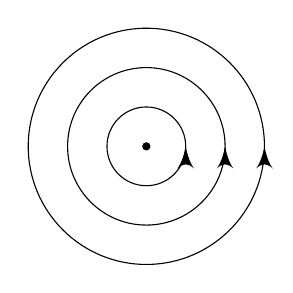
\begin{tikzpicture}
      \node [circ] {};
      \draw [->] circle [radius=0.5];
      \draw [->] circle [radius=1];
      \draw [->] circle [radius=1.5];
    \end{tikzpicture}
  \end{center}
  Since there is no radial velocity, we must have $\frac{\partial \phi}{\partial r} = 0$. So $\phi$ only depends on $\theta$. This corresponds to the solution $\phi = B\theta$.

  To find out the value of $B$, consider the circulation around a loop
  \[
    K = \oint_{r = a} \mathbf{u}\cdot \;\d \ell = \int_0^{2\pi} \frac{B}{a} \cdot a \;\d \theta = 2\pi B.
  \]
  So we get
  \[
    \phi = \frac{K}{2\pi}\theta,\quad u_\theta = \frac{K}{2\pi r}.
  \]
  It is an exercise for the reader to show that this flow is indeed irrotational, i.e.\ $\nabla \times \mathbf{u} = 0$ for $r \not= 0$, despite it looking rotational. Moreover, for any (simple) loop $c$, we get
  \[
    \oint_c \mathbf{u}\cdot\;\d \ell =
    \begin{cases}
      K & \text{the origin is inside C}\\
      0 & \text{otherwise}
    \end{cases}.
  \]
  We can interpret this as saying there is no vorticity everywhere, except at the singular point at the origin, where we have infinite vorticity. Indeed, we have
  \[
    \oint_c \mathbf{u}\cdot \d \ell = \int_S \boldsymbol\omega \cdot \mathbf{n} \;\d S,
  \]
  where $S$ is the surface bounded by $c$.
\end{eg}

\begin{eg}[Uniform flow past a cylinder]
  Consider the flow past a cylinder.
  \begin{center}
    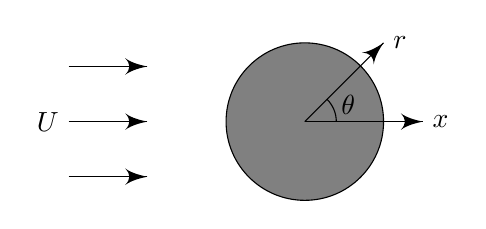
\begin{tikzpicture}
      \draw [fill=gray] circle [radius=1];
      \draw [->] (-3, 0.7) -- +(1, 0);
      \draw [->] (-3, 0) node [left] {$U$} -- +(1, 0);
      \draw [->] (-3, -0.7) -- +(1, 0);

      \draw [->] (0, 0) -- (1.5, 0) node [right] {$x$};
      \draw [->] (0, 0) -- (1, 1) node [right] {$r$};
      \draw (0.4, 0) arc(0:45:0.4) node [pos=0.7, right] {$\theta$};
    \end{tikzpicture}
  \end{center}
  We need to solve
  \begin{align*}
    \nabla^2 \phi &= 0 & r &> a\\
    \phi &\to U r\cos \theta & r & \to \infty\\
    \frac{\partial \phi}{\partial r} &= 0 & r &= a.
  \end{align*}
  We already have the general solution above. So we just write it down. We find
  \[
    \phi = U\left(r + \frac{a^2}{r}\right) \cos \theta + \frac{K}{2\pi}\theta.
  \]
  The last term allows for a net circulation $K$ around the cylinder, to account for vorticity in the viscous boundary layer on the surface of the cylinder. We have
  \begin{align*}
    u_r &= U\left(1 - \frac{a^2}{r^2}\right) \cos \theta\\
    u_\theta &= -U \left(1 + \frac{a^2}{r^2}\right) \sin \theta + \frac{K}{2 \pi r}.
  \end{align*}
  We can find the streamfunction for this as
  \[
    \psi = Ur\sin \theta\left(1 - \frac{a^2}{r^2}\right) - \frac{K}{2\pi} \log r.
  \]
  If there is no circulation, i.e.\ $K = 0$, then we get a flow similar to the flow around a sphere. Again, there is no net force on the cylinder, since flow is symmetric fore and aft, above and below. Again, we get two stagnation points at $A, A'$.
  \begin{center}
    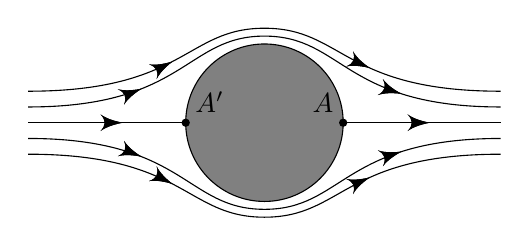
\begin{tikzpicture}
      \draw [->-=0.2, ->-=0.85] (-3, 0) -- (3, 0);
      \draw [fill=gray] circle [radius=1];
      \node [circ] at (-1, 0) {};
      \node [circ] at (1, 0) {};
      \node [anchor = south west] at (-1, 0) {$A'$};
      \node [anchor = south east] at (1, 0) {$A$};

      \draw [->-=0.23, ->-=0.8] (-3, 0.2) .. controls (-1, 0.2) and (-1, 1.1) .. (0, 1.1) .. controls (1, 1.1) and (1, 0.2) .. (3, 0.2);
      \draw [->-=0.3, ->-=0.73] (-3, 0.4) .. controls (-1, 0.4) and (-1, 1.2) .. (0, 1.2) .. controls (1, 1.2) and (1, 0.4) .. (3, 0.4);
      \draw [->-=0.23, ->-=0.8] (-3, -0.2) .. controls (-1, -0.2) and (-1, -1.1) .. (0, -1.1) .. controls (1, -1.1) and (1, -0.2) .. (3, -0.2);
      \draw [->-=0.3, ->-=0.73] (-3, -0.4) .. controls (-1, -0.4) and (-1, -1.2) .. (0, -1.2) .. controls (1, -1.2) and (1, -0.4) .. (3, -0.4);
    \end{tikzpicture}
  \end{center}
  What happens when $K \not= 0$ is more interesting. We first look at the stagnation points. We get $u_r = 0$ if and only if $r = a$ or $\cos \theta = 0$. For $u_\theta = 0$, when $r = a$, we require
  \[
    K = 4 \pi a U \sin \theta.
  \]
  So provided $|K| \leq 4 \pi a U$, there is a solution to this problem, and we get stagnation points on the boundary.
  \begin{center}
    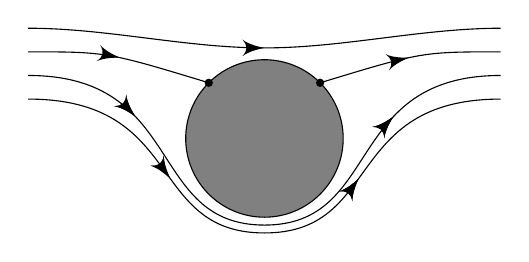
\begin{tikzpicture}
      \draw [fill=gray] circle [radius=1];
      \node [circ] at (-0.707, 0.707) {};
      \node [circ] at (0.707, 0.707) {};

      \draw [->-=0.5] (-3, 1.1) .. controls (-2, 1.1) .. (-0.707, 0.707);
      \draw [->-=0.5] (0.707, 0.707) .. controls (2, 1.1) .. (3, 1.1);
      \draw [->-=0.2, ->-=0.8] (-3, 0.8) .. controls (-1, 0.8) and (-1.5, -1.1) .. (0, -1.1) .. controls (1.5, -1.1) and (1, 0.8) .. (3, 0.8);
      \draw [->-=0.3, ->-=0.7] (-3, 0.5) .. controls (-1, 0.5) and (-1.5, -1.2) .. (0, -1.2) .. controls (1.5, -1.2) and (1, 0.5) .. (3, 0.5);

      \draw [->-=0.5] (-3, 1.4) .. controls (-2, 1.4) and (-1, 1.15) .. (0, 1.15) .. controls (1, 1.15) and (2, 1.4) .. (3, 1.4);
    \end{tikzpicture}
  \end{center}
  For $|K| > 4 \pi a U$, we do not get a stagnation point on the boundary. However, we still have the stagnation point where $\cos \theta = 0$, i.e.\ $\theta = \pm \frac{\pi}{2}$. Looking at the equation for $u_\theta = 0$, only $\theta = \frac{\pi}{2}$ works.
  \begin{center}
    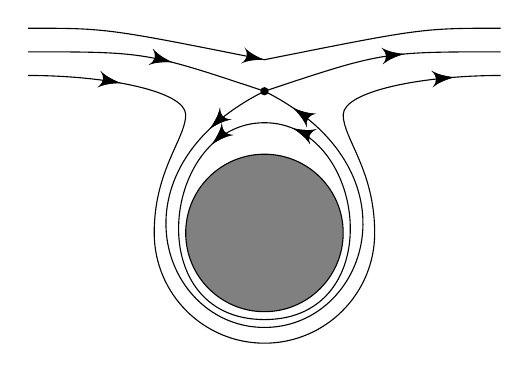
\begin{tikzpicture}
      \draw [fill=gray] circle [radius=1];
      \node [circ] at (0, 1.8) {};

      \draw [->-=0.1, ->-=0.95] (0, 1.8) .. controls (-2, 0.8) and (-1.3, -1.2) .. (0, -1.2) .. controls (1.3, -1.2) and (2, 0.8) .. (0, 1.8);

      \draw [->-=0.1, ->-=0.95] (0, 1.4) .. controls (-1.3, 1.4) and (-1.6, -1.1) .. (0, -1.1) .. controls (1.6, -1.1) and (1.3, 1.4) .. (0, 1.4);

      \draw [->-=0.3, ->-=0.8] (-3, 2.3) .. controls (-1.5, 2.3) .. (0, 1.8) .. controls (1.5, 2.3) .. (3, 2.3);

      \draw [->-=0.1, ->-=0.95] (-3, 2) .. controls (-2, 2) and (-1, 1.8) .. (-1, 1.5) .. controls (-1, 1.2) and (-1.4, 0.8) .. (-1.4, 0) arc (180:360:1.4) .. controls (1.4, 0.8) and (1, 1.2) .. (1, 1.5) .. controls (1, 1.8) and (2, 2) .. (3, 2);
      \draw [->-=0.5] (-3, 2.6) .. controls (-2, 2.6) .. (0, 2.2) .. controls (2, 2.6) and (2, 2.6) .. (3, 2.6);
    \end{tikzpicture}
  \end{center}
  Let's now look at the effect on the sphere. For steady potential flow, Bernoulli works (i.e.\ $H$ is constant) everywhere, not just along each streamline (see later). So we can calculate the pressure on the surface. Let $p$ be the pressure on the surface. Then we get
  \[
    p_\infty + \frac{1}{2} \rho U^2 = p + \frac{1}{2} \rho \left(\frac{K}{2\pi a} - 2U \sin \theta\right)^2.
  \]
  So we find
  \[
    p = p_\infty + \frac{1}{2} \rho U^2 - \frac{\rho K^2}{8 \pi^2 a^2} + \frac{\rho KU \sin \theta}{\pi a} - 2\rho U^2 \sin^2 \theta.
  \]
  We see the pressure is symmetrical fore and aft. So there is no force in the $x$ direction.

  However, we get a transverse force (per unit length) in the $y$-direction. We have
  \[
    F_y = -\int_0^{2\pi} p \sin \theta (a \;\d \theta) = -\int_0^{2\pi} \frac{\rho K U}{\pi a} \sin^2 \theta a \;\d \theta = - \rho UK.
  \]
  where we have dropped all the odd terms. So there is a sideways force in the direction perpendicular to the flow, and is directly proportional to the circulation of the system.

  In general, the \emph{magnus force} (lift force) resulting from interaction between the flow $\mathbf{U}$ and the vortex $\mathbf{K}$ is
  \[
    \mathbf{F} = \rho \mathbf{U}\times \mathbf{K}.
  \]
\end{eg}
\subsection{Time dependent potential flows}
Consider the time-dependent Euler equation
\[
  \rho\left(\frac{\partial \mathbf{u}}{\partial t} + \nabla\left(\frac{1}{2}|\mathbf{u}|^2\right) - \mathbf{u}\times \boldsymbol\omega\right) = -\nabla p - \nabla \chi.
\]
We assume that we have a potential flow $\mathbf{u} = \nabla \phi$. So $\boldsymbol\omega = 0$. Then we can write the whole equation as
\[
  \nabla \left(\rho \frac{\partial \phi}{\partial t} + \frac{1}{2} \rho |\mathbf{u}|^2 + p + \chi\right) = 0.
\]
Thus we can integrate this to obtain
\[
  \rho \frac{\partial\phi}{\partial t} + \frac{1}{2} \rho |\nabla \phi|^2 + p + \chi = f(t),
\]
where $f(t)$ is a function independent of space. This equation allows us to correlate the properties of $\phi$, $p$ etc. at different points in space.

\begin{eg}[Oscillations in a manometer]
  A manometer is a $U$-shaped tube.
  \begin{center}
    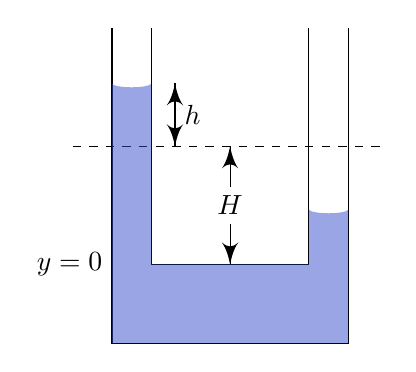
\begin{tikzpicture}
      \draw (0, 4) -- (0, 0) -- (3, 0) -- (3, 4);
      \draw (0.5, 4) -- (0.5, 1) -- (2.5, 1) -- (2.5, 4);
      \draw [dashed] (-0.5, 2.5) -- (3.5, 2.5);
      \draw [<->] (1.5, 1) -- (1.5, 2.5) node [pos=0.5, fill=white] {$H$};
      \node [left] at (0, 1) {$y = 0$};

      \fill [mblue, opacity=0.5] (0, 3.3) -- (0, 0) -- (3, 0) -- (3, 1.7) arc(0:-180:0.25 and 0.05) -- (2.5, 1) -- (0.5, 1) -- (0.5, 3.3) arc(0:-180:0.25 and 0.05);

      \draw [<->] (0.8, 2.5) -- (0.8, 3.3) node [pos=0.5, right] {$h$};
    \end{tikzpicture}
  \end{center}
  We use some magic to set it up such that the water level in the left tube is $h$ above the equilibrium position $H$. Then when we release the system, the water levels on both side would oscillate.

  We can get quite far just by doing dimensional analysis. There are only two parameters $g, H$. Hence the frequency must be proportional to $\sqrt{\frac{g}{H}}$. To get the constant of proportionality, we have to do proper calculations.

  We are going to assume the reservoir at the bottom is large, so velocities are negligible. So $\phi$ is constant in the reservoir, say $\phi = 0$. We want to figure out the velocity on the left. This only moves vertically. So we have
  \[
    \phi = uy = \dot{h}y.
  \]
  So we have
  \[
    \frac{\partial \phi}{\partial t} = \ddot{h}y.
  \]
  On the right hand side, we just have
  \[
    \phi = -uy = -\dot{g} y,\quad \frac{\partial \phi}{\partial t} = -\ddot{h}y.
  \]
  We now apply the equation from one tube to the other --- we get
  \begin{multline*}
    \rho \ddot{h} (H + h) + \frac{1}{2}\rho \dot{h}^2 + p_{\mathrm{atm}} + g\rho(H + h) = f(t) \\
    = -\rho\ddot{h}(H - h) + \frac{1}{2}\rho \dot{h}^2 + p_{\mathrm{atm}} + g\rho(H - h).
  \end{multline*}
  Quite a lot of these terms cancel, and we are left with
  \[
    2 \rho H\ddot{h} + 2g\rho h = 0.
  \]
  Simplifying terms, we get
  \[
    \ddot{h} + \frac{g}{H} h = 0.
  \]
  So this is simple harmonic motion with the frequency $\sqrt{\frac{g}{H}}$.
\end{eg}

\begin{eg}[Oscillations of a bubble]
  Suppose we have a spherical bubble of radius $a(t)$ in some fluid. Spherically symmetric oscillations induce a flow in the fluid. This satisfies
  \begin{align*}
    \nabla^2 \phi &= 0 & r & > a\\
    \phi&\to 0 & r &\to \infty\\
    \frac{\partial \phi}{\partial r} &= \dot{a} & r &= a.
  \end{align*}
  In spherical polars, we write Laplace's equation as
  \[
    \frac{1}{r^2} \frac{\partial}{\partial r} \left(r^2 \frac{\partial \phi}{\partial r}\right) = 0.
  \]
  So we have
  \[
    \phi = \frac{A(t)}{r},
  \]
  and
  \[
    u_r = \frac{\partial \phi}{\partial r} = -\frac{A(t)}{r^2}.
  \]
  This certainly vanishes as $r \to \infty$. We also know
  \[
    -\frac{A}{a^2} = \dot{a}.
  \]
  So we have
  \[
    \phi = -\frac{a^2\dot{a}}{r}.
  \]
  Now we have
  \[
    \left.\frac{\partial \phi}{\partial t}\right|_{r = a} = \left.-\frac{2a\dot{a}^2}{r} -\frac{a^2\ddot{a}}{r}\right|_{r = a} = -(a\ddot{a} + 2\dot{a}^2).
  \]
  We now consider the pressure on the surface of the bubble.

  We will ignore gravity, and apply Euler's equation at the bubble surface and at infinity. Then we get
  \[
    -\rho (a\ddot{a} + 2 \dot{a}^2) + \frac{1}{2}\rho \dot{a}^2 + p(a, t) = p_\infty.
  \]
  Hence we get
  \[
    \rho\left(a\ddot{a} + \frac{3}{2}\dot{a}^2\right) = p(a, t) - p_\infty.
  \]
  This is a difficult equation to solve, because it is non-linear. So we assume we have small oscillations about equilibrium, and write
  \[
    a = a_0 + \eta(t),
  \]
  where $\eta(t) \ll a_0$. Then we can write
  \[
    a\ddot{a} + \frac{3}{2} \dot{a}^2 = (a_0 + \eta) \ddot{\eta} + \frac{3}{2} \dot{\eta}^2 = a_0 \ddot{\eta} + O(\eta^2).
  \]
  Ignoring second order terms, we get
  \[
    \rho a_0 \ddot{\eta} = p(a, t) - p_\infty.
  \]
  We also know that $p_\infty$ is the pressure when we are in equilibrium. So $p(a, t) - p_\infty$ is the small change in pressure $\delta p$ caused by the change in volume.

  To relate the change in pressure with the change in volume, we need to know some thermodynamics. We suppose the oscillation is adiabatic, i.e.\ it does not involve any heat exchange. This is valid if the oscillation is fast, since there isn't much time for heat transfer. Then it is a \emph{fact} from thermodynamics that the motion obeys
  \[
    PV^\gamma =\text{ constant},
  \]
  where
  \[
    \gamma = \frac{\text{specific heat under constant pressure}}{\text{specific heat under constant volume}}.
  \]
  We can take logs to obtain
  \[
    \log p + \gamma \log V = \text{ constant}.
  \]
  Then taking small variations of $p$ and $V$ about $p_\infty$ and $V_0 = \frac{4}{3} \pi a_0^3$ gives
  \[
    \delta (\log p) + \gamma \delta(\log V) = 0.
  \]
  In other words, we have
  \[
    \frac{\delta p}{p_\infty} = -\gamma \frac{\delta V}{V_0}
  \]
  Thus we find
  \[
    p(a, t) - p_\infty = \delta p = -p_\infty \gamma \frac{\delta V}{V_0} = -3p_\infty\gamma \frac{\eta}{a_0}.
  \]
  Thus we get
  \[
    \rho a_0 \ddot{\eta} = -\frac{3 \gamma \eta}{a_0} p_\infty.
  \]
  This is again simple harmonic motion with frequency
  \[
    \omega = \left(\frac{3\gamma p_0}{\rho a_0}\right)^{1/2}.
  \]
  We know all these numbers, so we can put them in. For a $\SI{1}{\centi\meter}$ bubble, we get $\omega \approx \SI{2e3}{\per\second}$. For reference, the human audible range is $20 - \SI{20000}{\per\second}$. This is why we can hear, say, waves breaking.
\end{eg}

\section{Water waves}
We now consider water waves. We are first going to use dimensional analysis to understand the qualitative behaviour of water waves in deep and shallow water respectively. Afterwards, we will try to solve it properly, and see how we can recover the results from the dimensional analysis.
\begin{center}
  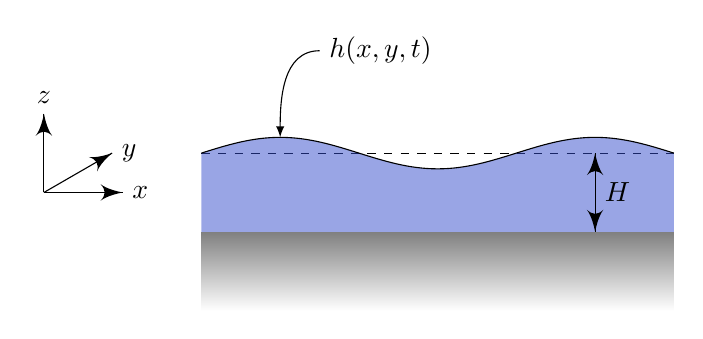
\begin{tikzpicture}
    \fill [gray, path fading=south] (-3, 0) rectangle (3, -1);

    \draw [dashed] (-3, 1) -- (3, 1);

    \fill [mblue, opacity=0.5] (-3, 0) -- (-3, 1) sin (-2, 1.2) cos (-1, 1) sin (0, 0.8) cos (1, 1) sin (2, 1.2) cos (3, 1) -- (3, 0) -- cycle;;

    \draw (-3, 1) sin (-2, 1.2) cos (-1, 1) sin (0, 0.8) cos (1, 1) sin (2, 1.2) cos (3, 1);

    \draw [->] (-5, 0.5) -- +(1, 0) node [right] {$x$};
    \draw [->] (-5, 0.5) -- +(0, 1) node [above] {$z$};
    \draw [->] (-5, 0.5) -- +(0.866, 0.5) node [right] {$y$};

    \draw (-1.5, 2.3) node [right] {$h(x, y, t)$} edge [out=180, in=90, -latex] (-2, 1.2);

    \draw [<->] (2, 0) -- (2, 1) node [pos=0.5, right] {$H$};
  \end{tikzpicture}
\end{center}
\subsection{Dimensional analysis}
Consider waves with wave number $k = \frac{2\pi}{\lambda}$, where $\lambda$ is the wavelength, on a layer of water of depth $H$. We suppose the fluid is inviscid. Then the wave speed $c$ depends on $k$, $g$ and $H$. Dimensionally, we can write the answer as
\[
  c = \sqrt{gH} f(kH).
\]
for some dimensionless function $f$.

Now suppose we have deep water. Then $H \gg \lambda$. Therefore $kH \gg 1$. In this limit, we would expect the speed not to depend on $H$, since $H$ is just too big. The only way this can be true is if
\[
  f \propto \frac{1}{\sqrt{kH}}.
\]
Then we know
\[
  c = \alpha \sqrt{\frac{g}{k}},
\]
where $\alpha$ is some dimensionless constant.

What happens near the shore? Here the water is shallow. So we have $kH \ll 1$. Since the wavelength is now so long, the speed should be independent of $k$. So $f$ is a constant, say $\beta$. So
\[
  c = \beta\sqrt{gH}.
\]
We don't know $\alpha$ and $\beta$. To know that, we would need proper theory. And we also need that to connect up the regimes of deep and shallow water, as we will soon do.

Yet these can already explain several phenomena we see in daily life. For example, we see that wave fronts are always parallel to the shore, regardless of how the shore is shaped and positioned. This is since if wave is coming in from an angle, the parts further away from the shore move faster (since it is deeper), causing the wave front to rotate until it is parallel.
\begin{center}
  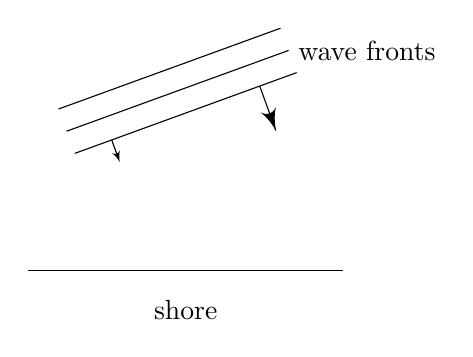
\begin{tikzpicture}
    \draw (-2, 0) -- (2, 0);
    \node at (0, -0.5) {shore};
    \begin{scope}[shift={(0, 2)}]
      \begin{scope}[rotate=20]
        \draw (-1.5, 0) -- (1.5, 0);
        \draw (-1.5, 0.3) -- (1.5, 0.3) node [right] {wave fronts};
        \draw (-1.5, 0.6) -- (1.5, 0.6);

        \draw [-latex'] (-1, 0) -- (-1, -0.3);
        \draw [->] (1, 0) -- (1, -0.6);
      \end{scope}
    \end{scope}
  \end{tikzpicture}
\end{center}
We can also use this to explain why waves break. Near the shore, the water is shallow, and the difference in height between the peaks and troughs of the wave is significant. Hence the peaks travels faster than the trough, causing the waves to break.
\begin{center}
  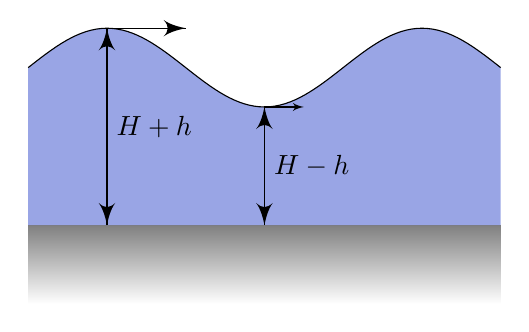
\begin{tikzpicture}
    \fill [gray, path fading=south] (-3, -1) rectangle (3, -2);

    \fill [mblue, opacity=0.5] (-3, -1) -- (-3, 1) sin (-2, 1.5) cos (-1, 1) sin (0, 0.5) cos (1, 1) sin (2, 1.5) cos (3, 1) -- (3, -1) -- cycle;;

    \draw (-3, 1) sin (-2, 1.5) cos (-1, 1) sin (0, 0.5) cos (1, 1) sin (2, 1.5) cos (3, 1);

    \draw [<->] (-2, -1) -- (-2, 1.5) node [pos=0.5, right] {$H + h$};
    \draw [<->] (0, -1) -- (0, 0.5) node [pos=0.5, right] {$H - h$};

    \draw [->] (-2, 1.5) -- +(1, 0);
    \draw [-latex'] (0, 0.5) -- +(0.5, 0);
  \end{tikzpicture}
\end{center}

\subsection{Equation and boundary conditions}
We now try to solve for the actual solution.
\begin{center}
  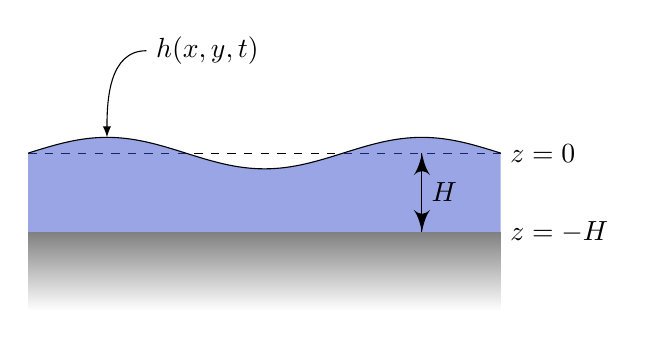
\begin{tikzpicture}
    \fill [gray, path fading=south] (-3, 0) rectangle (3, -1);

    \draw [dashed] (-3, 1) -- (3, 1) node [right] {$z = 0$};
    \node [right] at (3, 0) {$z = -H$};

    \fill [mblue, opacity=0.5] (-3, 0) -- (-3, 1) sin (-2, 1.2) cos (-1, 1) sin (0, 0.8) cos (1, 1) sin (2, 1.2) cos (3, 1) -- (3, 0) -- cycle;;

    \draw (-3, 1) sin (-2, 1.2) cos (-1, 1) sin (0, 0.8) cos (1, 1) sin (2, 1.2) cos (3, 1);

    \draw (-1.5, 2.3) node [right] {$h(x, y, t)$} edge [out=180, in=90, -latex] (-2, 1.2);

    \draw [<->] (2, 0) -- (2, 1) node [pos=0.5, right] {$H$};
  \end{tikzpicture}
\end{center}
We assume the fluid is inviscid, and the motion starts from rest. Thus the vorticity $\nabla \times \mathbf{u}$ is initially zero, and hence always zero. Together with the incompressibility condition $\nabla \cdot \mathbf{u} = 0$, we end up with Laplace's equation
\[
  \nabla^2 \phi = 0.
\]
We have some \emph{kinematic boundary conditions}. First of all, there can be no flow through the bottom. So we have
\[
  u_z = \frac{\partial \phi}{\partial z} = 0
\]
when $z = -H$. At the free surface, we have
\[
  u_z = \frac{\partial \phi}{\partial z} = \frac{\D h}{\D t} = \frac{\partial h}{\partial t} + u \frac{\partial h}{\partial x} + v \frac{\partial h}{\partial y}
\]
when $z = h$.

We then have the dynamic boundary condition that the pressure at the surface is the atmospheric pressure, i.e.\ at $z = h$, we have
\[
  p = p_0 = \text{constant}.
\]
We need to relate this to the flow. So we apply the time-dependent Bernoulli equation
\[
  \rho \frac{\partial \phi}{\partial t} + \frac{1}{2} \rho|\nabla \phi|^2 + g\rho h + p_0 = f(t)\text{ on }z = h.
\]
The equation is not hard, but the boundary conditions are. Apart from them being non-linear, there is this surface $h$ that we know nothing about.

It is impossible to solve these equations just as they are. So we want to make some approximations. We assume that the waves amplitudes are small, i.e.\ that
\[
  h \ll H.
\]
Moreover, we assume that the waves are relatively flat, so that
\[
  \frac{\partial h}{\partial x},\frac{\partial h}{\partial y} \ll 1,
\]
We then ignore quadratic terms in small quantities. For example, since the waves are small, the velocities $u$ and $v$ also are. So we ignore $u \frac{\partial h}{\partial x}$ and $v\frac{\partial h}{\partial y}$. Similarly, we ignore the whole of $|\nabla \phi|^2$ in Bernoulli's equations since it is small.

Next, we use Taylor series to write
\[
  \left.\frac{\partial \phi}{\partial z}\right|_{z = h} = \left.\frac{\partial \phi}{\partial z}\right|_{z = 0} + h \left.\frac{\partial^2 \phi}{\partial z^2}\right|_{z = 0} + \cdots.
\]
Again, we ignore all quadratic terms. So we just approximate
\[
  \left.\frac{\partial \phi}{\partial z}\right|_{z = h} = \left.\frac{\partial \phi}{\partial z}\right|_{z = 0}.
\]
We are then left with linear water waves. The equations are then
\begin{align*}
  \nabla^2 \phi &= 0 & -H < z &\leq 0\\
  \frac{\partial \phi}{\partial z} &= 0 & z &= -H\\
  \frac{\partial \phi}{\partial z} &= \frac{\partial h}{\partial t} & z &= 0\\
  \frac{\partial \phi}{\partial t} + gh &= f(t) & z &= h.
\end{align*}
Note that the last equation is just Bernoulli equations, after removing the small terms and throwing our constants and factors in to the function $f$.

We now have a nice, straightforward problem. We have a linear equation with linear boundary conditions, which we can solve.

\subsection{Two-dimensional waves (straight crested waves)}
We are going further simplify the situation by considering the case where the wave does not depend on $y$. We consider a simple wave form
\[
  h = h_0 e^{i(kx - \omega t)}.
\]
Using the boundary condition at $z = 0$, we know we must have a solution of the form
\[
  \phi = \hat{\phi}(z) e^{i(kx - \omega t)}.
\]
Putting this into Laplace's equation, we have
\[
  -k^2 \hat{\phi} + \hat{\phi}'' = 0.
\]
We notice that the solutions are then of the form
\[
  \hat{\phi} = \phi_0 \cosh k(z + H),
\]
where the constants are chosen so that $\frac{\partial \phi}{\partial z} = 0$ at $z = -H$.

We now have three unknowns, namely $h_0, \phi_0$ and $\omega$ (we assume $k$ is given, and we want to find waves of this wave number). We use the boundary condition
\[
  \frac{\partial \phi}{\partial z} = \frac{\partial h}{\partial t}\text{ at }z = 0.
\]
We then get
\[
  k \phi_0 \sinh kH = -i \omega h_0.
\]
We put in Bernoulli's equation to get
\[
  -i\omega \hat{\phi}(z) e^{i(kx - \omega t)} + g h_0 e^{i(kx - \omega t)} = f(t).
\]
For this not to depend on $x$, we must have
\[
  -i\omega \phi_0 \cosh kH + gh_0 = 0.
\]
The trivial solution is of course $h_0 = \phi_0 = 0$. Otherwise, we can solve to get
\[
  \omega^2 = gk \tanh kH.
\]
This is the \emph{dispersion relation}, and relates the frequency to the wavelengths of the wave.

We can use the dispersion relation to find the speed of the wave. This is just
\[
  c = \frac{\omega}{k} = \sqrt{\frac{g}{k}\tanh kH}.
\]
We can now look at the limits we have previously obtained with large and small $H$.

In deep water (or short waves), we have $kH \gg 1$. We know that as $kH \to \infty$, we get $\tanh kH \to 1$. So we get
\[
  c = \sqrt{\frac{g}{k}}.
\]
In shallow water, we have $kH \ll 1$. In the limit $kH \to 0$, we get $\tanh kH \to kH$. Then we get
\[
  c = \sqrt{gH}.
\]
This are exactly as predicted using dimensional analysis, with all the dimensionless constants being $1$.

We can now plot how the wave speed varies with $k$.
\begin{center}
  \begin{tikzpicture}[xscale=0.5]
    \draw [->] (-0.5, 0) -- (8, 0) node [right] {$kH$};
    \draw [->] (0, -0.5) -- (0, 2.5) node [right] {$\frac{c}{\sqrt{gH}}$};

    \node [circ] at (0, 2) {};
    \node [left] at (0, 2) {$1$};

    \draw [domain=0:8] plot [smooth] (\x, {2/(1 + \x^2/(3 + \x^2/(5 + \x^2/(7 + \x^2/(9 + \x^2/11)))))});
% continued fraction approximation to tanh x. Cannot use built in tanh x
% because (1) it does not work for large x; and (2) this avoids division by
% zero error when evaluating tanh x / x at x = 0 directly.
  \end{tikzpicture}
\end{center}
We see that wave speed decreases monotonically with $k$, and long waves travel faster than short waves.

This means if we start with, say, a square wave, the long components of the wave travels faster than the short components. So the square wave disintegrates as it travels.

Note also that this puts an upper bound on the maximum value of the speed $c$. There can be no wave travelling faster than $\sqrt{gH}$. Thus if you travel faster than $\sqrt{gH}$, all the waves you produce are left behind you. In general, if you have velocity $U$, we can define the \emph{Froude number}
\[
  Fr = \frac{U}{\sqrt{gH}}.
\]
This is like the Mach number.

For a tsunami, we have
\[
  \lambda \sim \SI{400}{\kilo\meter},\quad H \sim \SI{4}{\kilo\meter}.
\]
We are thus in the regime of small $kH$, and
\[
  c = \sqrt{10 \times 4\times 10^3} = \SI{200}{\meter\per\second}.
\]
Note that the speed of the tsunami depends on the depth of the water. So the topography of the bottom of the ocean will affect how tsunamis move. So knowing the topography of the sea bed allows us to predict how tsunamis will move, and can save lives.

\subsection{Group velocity}
Now suppose we have two waves travelling closely together with similar wave numbers, e.g.
\[
  \sin k_1 x + \sin k_2 x = 2 \sin \left(\frac{k_1 + k_2}{2} x\right) \cos\left(\frac{k_1 - k_2}{2}x\right),
\]
since $k_1$ and $k_2$ are very similar, we know $\frac{k_1 + k_2}{2} \approx k_1$, and $\frac{k_1 - k_2}{2}$ is small, hence the cosine term has long period. We would then expect waves to look like this
\begin{center}
  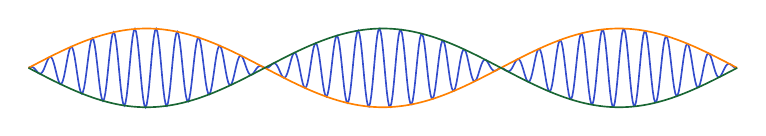
\begin{tikzpicture}[xscale=1.5]
    \draw [semithick, mblue, domain=0:6,samples=600] plot(\x, {0.5 * cos(2000 * \x) * sin (90 * \x)});
    \draw [semithick, morange] (0, 0) sin (1, 0.5) cos (2, 0) sin (3, -0.5) cos (4, 0) sin (5, 0.5) cos (6, 0);
    \draw [semithick, mgreen] (0, 0) sin (1, -0.5) cos (2, 0) sin (3, 0.5) cos (4, 0) sin (5, -0.5) cos (6, 0);
  \end{tikzpicture}
\end{center}
So the amplitudes of the waves would fluctuate. We say the wave travels in \emph{groups}. For more details, see IID Fluid Dynamics or IID Asymptotic methods.

It turns out the ``packets'' don't travel at the same velocity as the waves themselves. The group velocity is given by
\[
  c_g = \frac{\partial \omega}{\partial k}.
\]
In particular, for deep water waves, where $\omega \sim \sqrt{gk}$, we get
\[
  c_g = \frac{1}{2} \sqrt{\frac{g}{k}} = \frac{1}{2}c.
\]
This is also the velocity at which energy propagates.

\subsection{Rayleigh-Taylor instability}
Note that it is possible to turn the problem upside down, and imagine we have water over air:
\begin{center}
  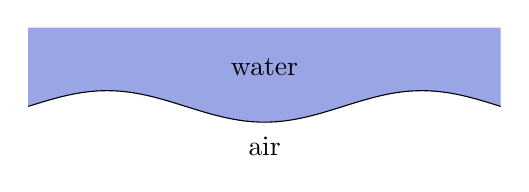
\begin{tikzpicture}
    \fill [mblue, opacity=0.5] (-3, 2) -- (-3, 1) sin (-2, 1.2) cos (-1, 1) sin (0, 0.8) cos (1, 1) sin (2, 1.2) cos (3, 1) -- (3, 2) -- cycle;;

    \draw (-3, 1) sin (-2, 1.2) cos (-1, 1) sin (0, 0.8) cos (1, 1) sin (2, 1.2) cos (3, 1);

    \node at (0, 1.5) {water};
    \node at (0, 0.5) {air};
  \end{tikzpicture}
\end{center}
We can imagine this as the same scenario as before, but with gravity pull upwards. So exactly the same equations hold, but we replace $-g$ with $g$. In deep water, we have
\[
  \omega^2 = -gk.
\]
So we have
\[
  \omega = \pm i\sqrt{gk}.
\]
Thus we get
\[
  h \propto A e^{\sqrt{gk} t} + B e^{-\sqrt{gk}t}.
\]
We thus have an exponentially growing solution. So the system is unstable, and water will fall down. This very interesting fact is known as \emph{Rayleigh-Taylor instability}.

\section{Fluid dynamics on a rotating frame}
We would like to study fluid dynamics in a rotating frame, because the Earth is rotating (hopefully). So this is particularly relevant if we want to study ocean currents or atmospheric flow.

\subsection{Equations of motion in a rotating frame}

The Lagrangian (particle) acceleration in a rotating frame of reference is given by
\[
  \frac{\D \mathbf{u}}{\D t} + 2 \boldsymbol\Omega \times \mathbf{u} + \boldsymbol\Omega \times (\boldsymbol\Omega \times \mathbf{x}),
\]
as you might recall from IA Dynamics and Relativity. So we have the equation of motion
\[
  \rho\left(\frac{\partial \mathbf{u}}{\partial t} + \mathbf{u}\cdot \nabla \mathbf{u} + 2 \boldsymbol\Omega \times \mathbf{u}\right) = -\nabla p - \rho \boldsymbol\omega \times (\boldsymbol\Omega \times \mathbf{x}) + \mathbf{g} \rho.
\]
This is complicated, so we want to simplify this. We will first compare the centrifugal force compared to gravity. We have
\[
  |\boldsymbol\Omega| = \frac{2\pi}{1\text{ day}} s^{-1} \approx \SI{2\pi e-5}{\per\second}.
\]
The largest scales are $\SI{10e4}{\kilo\meter}$. Compared to gravity $\mathbf{g}$, we have
\[
  \frac{|\boldsymbol\Omega \times (\boldsymbol\Omega \times \mathbf{x})|}{|\mathbf{g}|}\leq \frac{(2\pi)^2 \times 10^{-10}.\times 10^7}{10} \approx 4 \times 10^{-3}.
\]
So the centrifugal term is tiny compared to gravity, and we will ignore it. Alternatively, we can show that $\boldsymbol\Omega \times (\boldsymbol\omega \times \mathbf{x})$ can be given by a scalar potential, and we can incorporate it into the potential term, but we will not do that.

Next, we want to get rid of the non-linear terms. We consider motions for which
\[
  |\mathbf{u}\cdot \nabla \mathbf{u}| \ll |2 \boldsymbol\Omega \times \mathbf{u}|.
\]
The scales of these two terms are $U^2/L$ and $\Omega U$ respectively. So we need
\[
  R_o = \frac{U}{\Omega L} \ll 1.
\]
This is known as the Rossby number. In our atmosphere, we have $U \sim \SI{10}{\meter\per\second}$ and $L \sim \SI{1e3}{\kilo\meter}$. So we get
\[
  R_o = \frac{10}{10^6 \cdot 10^{-4}} \approx 0.1.
\]
So we can ignore the non-linear terms. Thus we get
\begin{prop}[Euler's equation in a rotating frame]
  \[
    \frac{\partial \mathbf{u}}{\partial t} + 2 \boldsymbol\Omega \times \mathbf{u} = -\frac{1}{\rho} \nabla p + \mathbf{g}.
  \]
\end{prop}

\begin{defi}[Coriolis parameter/planetary vorticity]
  We conventionally write $2 \boldsymbol\Omega = \mathbf{f}$, and we call this the \emph{Coriolis parameter} or the \emph{planetary vorticity}.
\end{defi}

Note that since we take the cross product of $\mathbf{f}$ with $\mathbf{u}$, only the component perpendicular to the velocity matters. Assuming that fluid flows along the surface of the earth, we only need the component of $\mathbf{f}$ normal to the surface, namely
\[
  f = 2 \Omega \sin \theta,
\]
where $\theta$ is the angle from the equator.
\subsection{Shallow water equations}
We are now going to derive the shallow water equations, where we have some water shallow relative to its horizontal extent. This is actually quite a good approximation for the ocean --- while the Atlantic is around $\SI{4}{\kilo\meter}$ deep, it is several thousand kilometers across. So the ratio is just like a piece of paper. Similarly, this is also a good approximation for the atmosphere.

Suppose we have a shallow layer of depth $z = h(x, y)$ with $p = p_0$ on $z = h$.
\begin{center}
  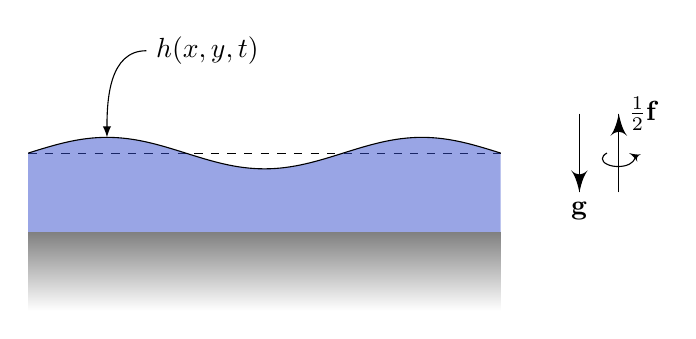
\begin{tikzpicture}
    \fill [gray, path fading=south] (-3, 0) rectangle (3, -1);

    \draw [dashed] (-3, 1) -- (3, 1);

    \fill [mblue, opacity=0.5] (-3, 0) -- (-3, 1) sin (-2, 1.2) cos (-1, 1) sin (0, 0.8) cos (1, 1) sin (2, 1.2) cos (3, 1) -- (3, 0) -- cycle;;

    \draw (-3, 1) sin (-2, 1.2) cos (-1, 1) sin (0, 0.8) cos (1, 1) sin (2, 1.2) cos (3, 1);

    \draw (-1.5, 2.3) node [right] {$h(x, y, t)$} edge [out=180, in=90, -latex] (-2, 1.2);

    \draw [->] (4, 1.5) -- +(0, -1) node [below] {$\mathbf{g}$};

    \draw [->] (4.5, 0.5) -- +(0, 1) node [right] {$\frac{1}{2} \mathbf{f}$};

    \draw [-latex'](4.35, 1) arc(135:405:0.2 and 0.1);
  \end{tikzpicture}
\end{center}
We consider motions with horizontal scales $L$ much greater than vertical scales $H$.

We use the fact that the fluid is incompressible, i.e.\ $\nabla \cdot \mathbf{u} = 0$. Writing $\mathbf{u} = (u, v, w)$, we get
\[
  \frac{\partial w}{\partial z} = -\frac{\partial u}{\partial x} - \frac{\partial v}{\partial y}.
\]
The scales of the terms are $W/H$, $U/L$ and $V/L$ respectively. Since $H \ll L$, we know $W \ll U, V$, i.e.\ most of the movement is horizontal, which makes sense, since there isn't much vertical space to move around.

We consider only horizontal velocities, and write
\[
  \mathbf{u} = (u, v, 0),
\]
and
\[
  \mathbf{f} = (0, 0, f).
\]
Then from Euler's equations, we get
\begin{align*}
  \frac{\partial u}{\partial t} - fv &= -\frac{1}{\rho} \frac{\partial p}{\partial x},\\
  \frac{\partial v}{\partial t} + fu &= -\frac{1}{\rho} \frac{\partial p}{\partial y},\\
  0 &= -\frac{1}{\rho}\frac{\partial p}{\partial z} -g.
\end{align*}
From the last equation, plus the boundary conditions, we know
\[
  p = p_0 = g\rho(h - z).
\]
This is just the hydrostatic balance. We now put this expression into the horizontal components to get
\begin{align*}
  \frac{\partial u}{\partial t} - fv &= -g\frac{\partial h}{\partial x},\\
  \frac{\partial v}{\partial t} + fu &= -g\frac{\partial h}{\partial y}.
\end{align*}
Note that the right hand sides are independent of $z$. So the accelerations are independent of $z$.

The initial conditions are usually that $u$ and $v$ are independent of $z$. So we assume that the velocities always do not depend on $z$.

\subsection{Geostrophic balance}
When we have steady flow, the time derivatives vanish. So we get
\begin{align*}
  u &= \pd{y} \left(-\frac{gh}{f}\right) = \pd{y} \left(-\frac{p}{\rho f}\right),\\
  v &= -\pd{x} \left(-\frac{gh}{f}\right) = -\pd{x} \left(-\frac{p}{\rho f}\right).
\end{align*}
Hopefully, this reminds us of streamfunctions. The streamlines are places where $h$ is constant, i.e.\ the surface is of constant height, i.e.\ the pressure is constant.

\begin{defi}[Shallow water streamfunction]
  The quantity
  \[
    \psi = -\frac{gh}{f}
  \]
  is the \emph{shallow water streamfunction}.
\end{defi}

In general, near a low pressure zone, there is a pressure gradient pushing the flow towards to the low pressure area. Since flow moves in circles around the low pressure zone, there is a Coriolis force that balances this force. This is the geostrophic balance.
\begin{center}
  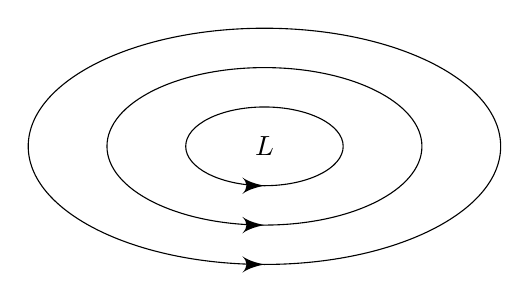
\begin{tikzpicture}
    \node {$L$};
    \draw [->-=0.75] ellipse (1 and 0.5);
    \draw [->-=0.75] ellipse (2 and 1);
    \draw [->-=0.75] ellipse (3 and 1.5);
  \end{tikzpicture}
\end{center}
This is a cyclone. Note that this picture is only valid in the Northern hemisphere. If we are on the other side of the Earth, cyclones go the other way round.

We now look at the continuity equation, i.e.\ the conservation of mass.

We consider a horizontal surface $\mathcal{D}$ in the water. Then we can compute
\[
  \frac{\d}{\d t} \int_\mathcal{D} \rho h \;\d V = -\int_{\partial \mathcal{D}} h \rho \mathbf{u}_H \cdot \mathbf{n}\;\d S,
\]
where $\mathbf{u}_H$ is the horizontal velocity. Applying the divergence theorem, we get
\[
  \int_{\mathcal{D}} \pd{t} (\rho h)\;\d V = -\int_{\mathcal{D}} \nabla_H \cdot (\rho h \mathbf{u}_H)\;\d V,
\]
where
\[
  \nabla_H = \left(\pd{x}, \pd{y}, 0\right).
\]
Since this was an arbitrary surface, we can take the integral away, and we have the continuity equation
\[
  \frac{\partial h}{\partial t} + \nabla_H \cdot (\mathbf{u}_h h) = 0.
\]
So if there is water flowing into a point (i.e.\ a vertical line), then the height of the surface falls, and vice versa.

We can write this out in full. In Cartesian coordinates:
\[
  \frac{\partial h}{\partial t} + \frac{\partial}{\partial x}(uh) + \pd{y}(uh) = 0.
\]
To simplify the situation, we suppose we have small oscillations, so we have $h = h_0 + \eta(x, y, t)$, where $\eta \ll h_0$, and write
\[
  \mathbf{u} = (u(x, y), v(x, y)).
\]
Then we can rewrite our equations of motion as
\[
  \frac{\partial \mathbf{u}}{\partial t} + \mathbf{f} \times \mathbf{u} = -g \nabla \eta\tag{$*$}
\]
and, ignoring terms like $u\eta, v\eta$, the continuity equation gives
\[
  \frac{\d \eta}{\d t} + h_0 \nabla \cdot \mathbf{u} = 0.\tag{$\dagger$}
\]
Taking the curl of the $(*)$, we get
\[
  \frac{\partial \boldsymbol\zeta}{\partial t} + \mathbf{f}\nabla \cdot \mathbf{u} = 0,
\]
where
\[
  \boldsymbol\zeta = \nabla \times \mathbf{u}.
\]
Note that even though we wrote this as a vector equation, really only the $z$-component is non-zero. So we can also view $\boldsymbol\zeta$ and $\mathbf{f}$ as scalars, and get a scalar equation.

We can express $\nabla \cdot \mathbf{u}$ in terms of $\eta$ using $(\dagger)$. So we get
\[
  \frac{\partial}{\partial t}\left(\boldsymbol\zeta - \frac{\eta}{h_0}\mathbf{f}\right) = \frac{\d \mathbf{Q}}{\d t} = 0,
\]
where
\begin{defi}[Potential vorticity]
  The \emph{potential vorticity} is
  \[
    \mathbf{Q} = \boldsymbol\zeta - \frac{\eta}{h_0}\mathbf{f},
  \]
\end{defi}
and this is conserved.

Hence given any initial condition, we can compute $\mathbf{Q}(x, y, 0) = \mathbf{Q}_0$. Then we have
\[
  \mathbf{Q}(x, y, t) = \mathbf{Q}_0
\]
for all time.

How can we make use of this? We start by taking the divergence of $(*)$ above to get
\[
  \frac{\partial}{\partial t}(\nabla \cdot \mathbf{u}) - \mathbf{f} \cdot \nabla \times \mathbf{u} = - g \nabla^2 \eta,
\]
and use $(\dagger)$ to substitute
\[
  \nabla \cdot \mathbf{u} = -\frac{1}{h_0} \frac{\partial \eta}{\partial t}.
\]
We then get
\[
  -\frac{1}{h_0} \frac{\partial^2 \eta}{\partial t^2} - \mathbf{f}\cdot \boldsymbol\zeta = -g\nabla^2 \eta.
\]
We now use the conservation of potential vorticity, namely
\[
  \boldsymbol\zeta = \mathbf{Q}_0 + \frac{\eta}{h_0}\mathbf{f},
\]
to rewrite this as
\[
  \frac{\partial^2 \eta}{\partial t^2} - gh_0 \nabla^2 \eta + \mathbf{f}\cdot \mathbf{f} \eta = - h_0 \mathbf{f}\cdot \mathbf{Q}_0.
\]
Note that the right hand side is just a constant (in time). So we have a nice differential equation we can solve.

\begin{eg}
  Suppose we have fluid with mean depth $h_0$, and we start with the following scenario:
  \begin{center}
    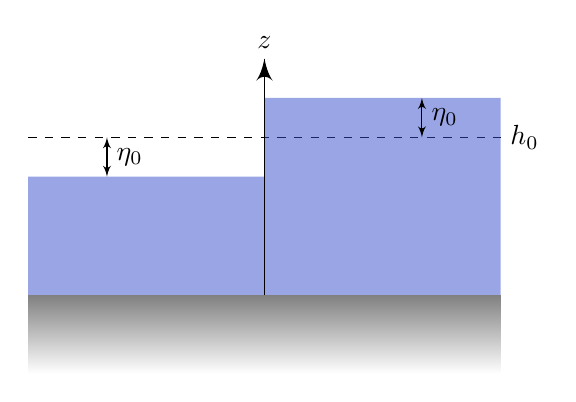
\begin{tikzpicture}
      \fill [gray, path fading=south] (-3, 0) rectangle (3, -1);

      \draw [dashed] (-3, 2) -- (3, 2) node [right] {$h_0$};
      \fill [mblue, opacity=0.5] (-3, 0) -- (-3, 1.5) -- (0, 1.5) -- (0, 2.5) -- (3, 2.5) -- (3, 0) -- cycle;

      \draw [latex'-latex'] (2, 2) -- +(0, 0.5) node [right, pos=0.5] {$\eta_0$};
      \draw [latex'-latex'] (-2, 2) -- +(0, -0.5) node [right, pos=0.5] {$\eta_0$};

      \draw [->] (0, 0) -- (0, 3) node [above] {$z$};
    \end{tikzpicture}
  \end{center}
  Due to the differences in height, we have higher pressure on the right and lower pressure on the left.

  If there is no rotation, then the final state is a flat surface with no flow. However, this cannot be the case if there is rotation, since this violates the conservation of $\mathbf{Q}$. So what happens if there is rotation?

  At the beginning, there is no movement. So we have $\boldsymbol\zeta(t = 0) = 0$. Thus we have
  \[
    Q_0 =
    \begin{cases}
      -\frac{\eta_0}{h_0}f & x > 0\\
      \frac{\eta_0}{h_0}f & x < 0
    \end{cases}.
  \]
  We seek the final steady state such that
  \[
    \frac{\partial \eta}{\partial t} = 0.
  \]
  We further assume that the final solution is independent of $y$, so
  \[
    \frac{\partial \eta}{\partial y} = 0.
  \]
  So $\eta = \eta(x)$ is just a function of $x$. Our equation then says
  \[
    \frac{\partial^2 \eta}{\partial x^2} - \frac{f^2}{gh_0} \eta = \frac{f}{g}Q_0 = \mp \frac{f^2}{gh_0}\eta_0.
  \]
  It is convenient to define a new variable
  \[
    R = \frac{\sqrt{gh_0}}{f},
  \]
  which is a length scale. We know $\sqrt{gh_0}$ is the fastest possible wave speed, and thus $R$ is how far a wave can travel in one rotation period. We rewrite our equation as
  \[
    \frac{\d^2 \eta}{\d x^2} - \frac{1}{R^2}\eta = \mp \frac{1}{R^2}\eta_0.
  \]
  \begin{defi}[Rossby radius of deformation]
    The length scale
    \[
      R = \frac{\sqrt{gh_0}}{f}
    \]
    is the \emph{Rossby radius of deformation}.
  \end{defi}
  This is the fundamental length scale to use in rotating systems when gravity is involved as well.

  We now impose our boundary conditions. We require $\eta \to \pm \eta_0$ as $x \to \pm \infty$. We also require $\eta$ and $\frac{\d \eta}{\d x}$ to be continuous at $x = 0$.

  The solution is
  \[
    \eta = \eta_0
    \begin{cases}
      1 - e^{-x/R} & x > 0\\
      -(1 - e^{x/R}) & x < 0
    \end{cases}.
  \]
  We can see that this looks quite different form the non-rotating case. It looks like this:
  \begin{center}
    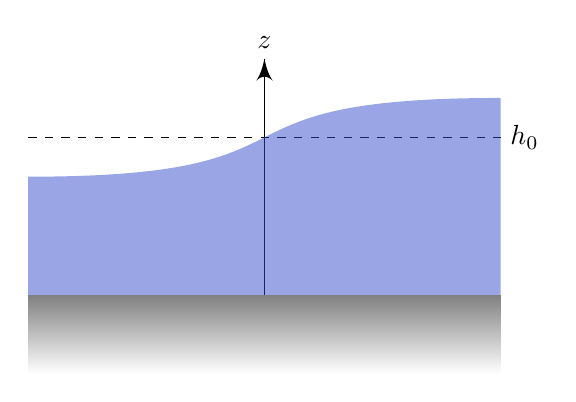
\begin{tikzpicture}
      \fill [gray, path fading=south] (-3, 0) rectangle (3, -1);
      \draw [->] (0, 0) -- (0, 3) node [above] {$z$};

      \draw [dashed] (-3, 2) -- (3, 2) node [right] {$h_0$};
      \fill [mblue, opacity=0.5] (-3, 0) -- (-3, 1.5) .. controls (1, 1.5) and (-1, 2.5) .. (3, 2.5) -- (3, 0) -- cycle;
    \end{tikzpicture}
  \end{center}
  The horizontal length scale involved is $2R$.

  We now look at the velocities. Using the steady flow equations, we have
  \begin{align*}
    u &= -\frac{g}{f} \frac{\partial \eta}{\partial y} = 0\\
    v &= \frac{g}{f} \frac{\partial\eta}{\partial x} = \eta_0 \sqrt{\frac{g}{h_0}} e^{-|x|/R}.
  \end{align*}
  So there is still flow in this system, and is a flow in the $y$ direction into the paper. This flow gives Coriolis force to the right, and hence balances the pressure gradient of the system.

  The final state is not one of rest, but one with motion in which the Coriolis force balances the pressure gradient. This is geostrophic flow.
\end{eg}

Going back to our pressure maps, if we have high and low pressure systems, we can have flows that look like this:
\begin{center}
  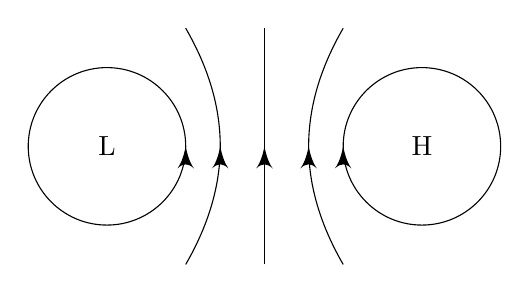
\begin{tikzpicture}
    \node {L};

    \node at (4, 0) {H};

    \draw [->] circle [radius=1];
    \draw [-<-=0.5] (4, 0) circle [radius=1];

    \draw (1, -1.5) edge [out=60,in=-60, ->-=0.5] (1, 1.5);
    \draw (3, -1.5) edge [out=120,in=-120, ->-=0.5] (3, 1.5);

    \draw [->-=0.5] (2, -1.5) -- (2, 1.5);
  \end{tikzpicture}
\end{center}
Then the Coriolis force will balance the pressure gradients.

So weather maps describe balanced flows. We can compute the scales here. In the atmosphere, we have approximately
\[
  R \approx \frac{\sqrt{10 \cdot 10^3}}{10^{-4}} = 10^6 \approx \SI{1000}{\kilo\meter}.
\]
So the scales of cyclones are approximately $\SI{1000}{\kilo\meter}$.

On the other hand, in the ocean, we have
\[
  R \approx \frac{\sqrt{10 \cdot 10}}{10^{-4}} = 10^5 = \SI{100}{\kilo\meter}.
\]
So ocean scales are much smaller than atmospheric scales.
\end{document}
